
\documentclass[
	ngerman          % neue deutsche Rechtschreibung
	,a4paper          % Papiergrösse
	% ,twoside          % Zweiseitiger Druck (rechts/links)
	,12pt             % Schriftgrösse (11pt default in Vorlage)
	,pdftex
	,abstract=on
	%  ,hidelinks		% Kästchen um Links verbergen
	%  ,disable         % Todo-Markierungen auschalten
	]{scrreprt}
\setcounter{tocdepth}{1} % Tiefe der TOC, Chapter starten bei 0

\usepackage{styles/bericht}
\usepackage{adjustbox}
\usepackage{paralist}
\usepackage{appendix}


\newcommand{\Autor}{\textcolor{red}{Dein Name}} %TODO Namen angeben
\newcommand{\Abschluss}{Bachelor of Science}
\newcommand{\Studiengang}{Informatik}
\newcommand{\MatrikelNummer}{\textcolor{red}{Deine Matrikelnummer}} %TODO Matrikelnummer angeben
\newcommand{\Kursbezeichnung}{TINF17B5}

\newcommand{\FirmenName}{\textcolor{red}{Deine Firma}} %TODO Firma angeben
\newcommand{\FirmenStadt}{\textcolor{red}{Dein Firmenstandort}} %TODO Firmenstandort angeben

%TODO Firmenlogo ändern
\newcommand{\FirmenLogoDeckblatt}
			{
\includegraphics[width=4cm]{images/Logos/firmen-logo}}
\newcommand{\DHBWLogoDeckblatt}
			{
\includegraphics[width=4cm]{images/Logos/dhbw-logo}}


%%%%%%%%
%%%% Veränderliche Daten
%%%%%%%%%%%%%%%%%%%%%%%%%%%%%%%%%%%%%%%%%%%%%%%%%%%%%%%%%%%
\newcommand{\BetreuerFirma}{\textcolor{red}{Betreuer}} %TODO Betreuer definieren
\newcommand{\BerichtArt}{\textcolor{red}{Berichtart}} %TODO Art definieren

\newcommand{\Titel}{\textcolor{red}{Titel}} %TODO Titel definieren
\newcommand{\AbgabeDatum}{\textcolor{red}{Abgabedatum}} %TODO Abgabedatum definieren

\newcommand{\Dauer}{\textcolor{red}{Bearbeitungszeitraum}} %TODO: Bearbeitungszeitraum


\hypersetup{%%
	pdfauthor={\Autor},
	pdftitle={\Titel},
	pdfsubject={\BerichtArt}
}

%%% Schrift definition
%%%%%%%%%%%%%%%%%%%%%%%%%%%%
\usepackage[onehalfspacing]{setspace}
% Times new Roman
%\usepackage{mathptmx} \renewcommand{\familydefault}{\rmdefault}
% Arial
%\usepackage{uarial} \renewcommand{\familydefault}{\sfdefault}
% Computern-Modern Schriftfamilie
\usepackage{lmodern}

\usepackage{color, colortbl}
\definecolor{Gray}{gray}{0.9}


%%% Paragraph-Überschrift in extra Zeile
%%%%%%%%%%%%%%%%%%%%%%%%%%%%
\makeatletter
\renewcommand\paragraph{\@startsection{paragraph}{4}{\z@}%
	{-3.25ex\@plus -1ex \@minus -.2ex}%
	{1.5ex \@plus .2ex}%
	{\normalfont\normalsize\bfseries}}
\makeatother



%%% Tabelle: Abstände (Spalte / Zeile)
%%%%%%%%%%%%%%%%%%%%%%%%%%%%
\setlength{\tabcolsep}{6pt} % Default value: 6pt
\renewcommand{\arraystretch}{1.5} % Default value: 1

%%% Tabelle: Neue Fixed-Width Spaltentypen
%%%%%%%%%%%%%%%%%%%%%%%%%%%%
\newcolumntype{L}[1]{>{\raggedright\let\newline\\\arraybackslash\hspace{0pt}}m{#1}}
\newcolumntype{C}[1]{>{\centering\let\newline\\\arraybackslash\hspace{0pt}}m{#1}}
\newcolumntype{R}[1]{>{\raggedleft\let\newline\\\arraybackslash\hspace{0pt}}m{#1}}


%%%%%%%%%%%%%%%%%%%%%%%%%%%%%%%%%%%%%%%%%%%%%%%
%% Neue Befehle (Mario)
%%%%%%%%%%%%%%%%%%%%%%%%%%%%%%%%%%%%%%%%%%%%%%%
\newcommand\tab[1][1cm]{\hspace*{#1}}




%%%%%%%%%%%%%%%%%%%%%%%%%%%%%%%%%%%%%%%%%%%%%%%%%%%%%%%%%%%%%%%%%%%%%%%%%%%%%%%

% Benutzt man das "biblatex"-Paket, dann muß das hier stehen:
% siehe auch die mit BIBLATEX markierten Zeil bericZählert.sty

\begin{document}
	\pagenumbering{Roman}
	%%%%%%%%%%%%%%%%%%%%%%%%%%%%%%%%%%%%%%%%%%%%%%%%%%%%%%%%%%%%%%%%%%%%%%%%%%%%%%%
	
	\begin{titlepage}
		
\begin{center}
	\vspace*{-2cm}
	\hfill\DHBWLogoDeckblatt\\[1.5cm]
	{\LARGE \Titel}\\[1.5cm]
	{\LARGE\scshape \BerichtArt}\\[1.5cm]
	{\large für die Prüfung zum}\\[0.5cm]
	{\Large \Abschluss}\\[0.5cm]
	{\large des Studienganges \Studiengang}\\[0.3cm]
	{\large an der}\\[0.3cm]
	{\large Dualen Hochschule Baden-Württemberg Karlsruhe}\\[0.3cm]
	{\large von}\\[0.5cm]
	{\large\bfseries \Autor}\\[1cm]
	{\large Abgabedatum \AbgabeDatum}
	\vfill

\begin{tabular}{l@{\hspace{2cm}}l}
	%Bearbeitungszeitraum			& \Dauer 			\\
	Matrikelnummer					& \MatrikelNummer		\\
	Kurs							& \Kursbezeichnung		\\
	Ausbildungsfirma				& \FirmenName			\\
									& \FirmenStadt			\\
	%Betreuer der Ausbildungsfirma	& \BetreuerFirma		\\
\end{tabular}
\end{center}
	\end{titlepage}
	
	%%%%%%%%%%%%%%%%%%%%%%%%%%%%%%%%%%%%%%%%%%%%%%%%%%%%%%%%%%%%%%%%%%%%%%%%%%%%%%%
	
	% Nur für Bachelorarbeiten einfügen:
	%%%%%%%%%%%%%%%%%%%%%%%%%%%%%%%%%%%%%%%%%%%%%%%%%%%%%%%%%%%%%%%%%%%%%%%%%%%%%%%
%% Descr:       Vorlage für Berichte der DHBW-Karlsruhe, Erklärung
%% Author:      Prof. Dr. Jürgen Vollmer, vollmer@dhbw-karlsruhe.de
%% $Id: erklaerung.tex,v 1.6 2016/03/16 12:51:09 vollmer Exp $
%% -*- coding: utf-8 -*-
%%%%%%%%%%%%%%%%%%%%%%%%%%%%%%%%%%%%%%%%%%%%%%%%%%%%%%%%%%%%%%%%%%%%%%%%%%%%%%%

% In Bachelorarbeiten muss eine schriftliche Erklärung abgegeben werden.
% Hierin bestätigen die Studierenden, dass die Bachelorarbeit, etc.
% selbständig verfasst und sämtliche Quellen und Hilfsmittel angegeben sind. Diese Erklärung
% bildet das zweite Blatt der Arbeit. Der Text dieser Erklärung muss auf einer separaten Seite
% wie unten angegeben lauten.

\thispagestyle{empty}
\begin{framed}
	\begin{center}
		\Large\bfseries Erklärung
	\end{center}

	\medskip
	\noindent
	Ich versichere hiermit, dass ich meinen \BerichtArt{} mit
	dem Thema:\\ 
	\begin{center}
	\enquote{\Titel}\\
	\end{center}
	selbstständig verfasst und keine anderen als die angegebenen Quellen und
	Hilfsmittel benutzt habe. Ich versichere zudem, dass die eingereichte elektronische Fassung mit der
	gedruckten Fassung übereinstimmt.
	
	\vspace{3cm}
	\noindent
	\underline{\hspace{6cm}}\hfill\underline{\hspace{6cm}}\\
	Ort~~~~~~~~~~~~Datum\hfill Unterschrift\hspace{4cm}
\end{framed}


%%%%%%%%%%%%%%%%%%%%%%%%%%%%%%%%%%%%%%%%%%%%%%%%%%%%%%%%%%%%%%%%%%%%%%%%%%%%%%%
\endinput
%%%%%%%%%%%%%%%%%%%%%%%%%%%%%%%%%%%%%%%%%%%%%%%%%%%%%%%%%%%%%%%%%%%%%%%%%%%%%%%

	
\begin{abstract}
	\todo[inline]{Zusammenfassung}
\end{abstract}
	\newcounter{savepage}
	
	
\tableofcontents           % Inhaltsverzeichnis hier ausgeben
\listoffigures             % Liste der Abbildungen
\listoftables              % Liste der Tabellen
%\lstlistoflistings         % Liste der Listings
%\listofequations           % Liste der Formeln

%%%%%%%%%%%%%%%%%%%%%%%%%%%%%%%%%%%%%%%%%%%%%%%%%%%%%%%%%%%%%%%%%%%%%%%%%%%%%%
%% Descr:       Vorlage für Berichte der DHBW-Karlsruhe, Datei mit Abkürzungen
%% Author:      Prof. Dr. Jürgen Vollmer, vollmer@dhbw-karlsruhe.de
%% $Id: abk.tex,v 1.3 2016/03/16 12:21:40 vollmer draft $
%% -*- coding: utf-8 -*-
%%%%%%%%%%%%%%%%%%%%%%%%%%%%%%%%%%%%%%%%%%%%%%%%%%%%%%%%%%%%%%%%%%%%%%%%%%%%%%%

\chapter*{Abkürzungsverzeichnis}


\begin{acronym}[DHBW]
	% \acro{Name}{Darstellung der Abkürzung}{Langform der Abkürzung}
	
\end{acronym}
 % Abkürzungsverzeichnis
	
	%Hier startet der Inhalt -> Arabische Seitennummerierung
	\setcounter{savepage}{\arabic{page}}
	\pagenumbering{arabic}
	\chapter{Einleitung}

\section{Projektumfeld}

\section{Motivation}

\section{Aufgabenstellung}

	\paragraph{Abgrenzung}


\section{Methodisches Vorgehen}

	\chapter{Grundlagen}
\section{Bildkompression}
Für die Anwendung der \acl{ELA} zu verstehen, ist es wichtig die Grundlagen der Bildkompression zu kennen. Die \ac{ELA} setzt an den Eigenschaften an, welche Bilder in Verlustbehafteten Bildformaten aufweisen.\\
Eines der bekanntesten Bildformate welches diese Eigenschaft ausweist ist JPEG, eine Norm (ISO/IEC 10918-1 oder CCITT T.81) zur Bildkomprimierung welche von der \ac{JPEG} entwickelt wurde. Das \ac{JPEG}-Schema ist zwar bei genauer Betrachtung recht komplex, das Grundprinzip ist allerdings leicht zu verstehen.\\
In einem ersten Schritt wird das Bitmap-Bild in 8x8 Matrizen aufgeteilt und mit Hilfe der \acp{DCT} von einer 8x8 Ortsmatrix, in eine 8x8 Frequenzmatrix umgewandelt. Alle folgenden Schritte arbeiten nun mit der diesen Matrizen, das Bild wird nicht mehr als ganzes betrachtet.\\
Jede dieser Pixelgruppen wird separat mit einer eigenen DCT kodiert und kann auch wieder verlustfrei reproduziert werden. Abbildung \ref{fig:Dctjpeg} zeigt die Basisfunktion einer zweidimensionalen DCT (Quantisierungstabelle) wobei zu sehen ist, dass die Frequenz von links nach rechts und von oben nach unten zunimmt. Bei der anschließenden Quantisierung werden die höherfrequenten Anteile des Bildes geringer gewichtet, als die niederfrequenten und die Koeffizienten welche nahezu 0 sind werden auf 0 gesetzt.\cite{Zichner2002}
Der letzte Schritt der Kompression ist die Entropie-Kodierung der Koeffizienten, wobei hier meistens die Huffman-Kodierung zum Einsatz kommt.\\
Die Dateigröße des komprimierten Bildes hängt vom Inhalt und der Qualität des Originalbildes ab. In der Regel benötigt ein Bild mit wenig Details wie zum Beispiel einem Foto des blauen Himmels weniger Speicherplatz als ein Bild welches viele Details enthält wie z.B. ein Foto einer Menschenmenge.\cite{Warif_2015}\\

\begin{figure}[H]
	\begin{center}
		
\includegraphics[scale=0.4]{images/Dctjpeg.png}
		\caption{Basisfunktion einer zweidimensionalen DCT (Quantisierungstabelle)}
		\label{fig:Dctjpeg}
	\end{center}
\end{figure}

\section{Erkennung von Kompressionsartefakten}
In den meisten Fällen einer Bildmanipulation wird ein Bild neu komprimiert, speziell dann wenn es durch die Bildbearbeitungssoftware abgespeichert wird. Dieser Vorgang verändert die ursprüngliche Komprimierungseigenschaften, das Ziel besteht nun darin diese Komprimierungseigenschaften, auch Artefakte genannt, zu analysieren und innerhalb eines Bildes möglicherweise Inkonsistenzen zu erkennen.\\
Hier gibt es zwei methodische Vorgehensweisen um solche Artefakte zu unterscheiden. Erstere Methode versucht Inkonsistenzen in der JPEG-Quantisierungstabellen zu erkennen, zweitere verwendet die Komprimierungsartefakte im Frequenzbereich des Bildes um so eine Signatur zu bilden und zwischen unterschiedlichen Kompressionscharakteristika zu unterscheiden.\cite{Chen2011} In folgenden Unterpunkten werden beide Ansätze nochmals kurz zusammengefasst:

\subsection{Inkonsistenz bei der Quantisierungstabelle}
Beim kodieren eines JPEG Bildes werden alle 8x8 Blöcke bei der Entropie-Kodierung durch dieselbe Quantisierungstabelle kodiert. Wenn nun ein Manipuliertes Bild vorliegt können Bereiche dessen, Eigenschaften von verschiedenen Quantisierungstabellen enthalten was zu einer Inkonsistenz führt. Zur Schätzung der Quantisierungstabelle des Originalbildes bei JPEG gibt es mehrere mathematische Verfahren welche anwendbar sind: Gängig ist unter anderem die Maximum-Likelihood-Schätzung auch als \emph{Methode der größten Plausibilität} bezeichnet oder die Maximum-a-posteriori-Schätzung.\cite{Chen2011} Auf die mathematischen Schätzverfahren wird nicht weiter Bezug genommen.\\
Mit der geschätzten Quantisierungstabelle ist es nun möglich, Blockinkonsistenzen zu erkennen und die Blöcke welche von einer Bildmanipulation betroffen sind zu lokalisieren. Die Möglichkeit, dass die Schätzung stark von der verwendeten Quantisierungstabelle des Originalbildes abweicht erhöht sich aber mit jeder erneuten Kompression des Manipulierten Bildes.\\
In der Praxis findet eine erneute Kompression einer Manipulation meist nicht durch den Ersteller sondern durch das verwendete Medium statt. So werden in den allermeisten sozialen Netzwerken Bilder nach dem Hochladen erneut komprimiert um die Dateigröße zu verringern und so Zeit beim erneuten Abruf über das Netzwerk zu sparen. Auch die gängigen Messenger-Dienste komprimieren das Bild vor dem Absenden. Eine bessere Erkennung von mehrfach komprimierten Bildern liefert die Methode welche im nächsten Unterpunkt beschrieben wird.



\subsection{Anomalie von Kompressionsartefakten}
	
\chapter{Implementierung}
Eine Implementierung eines Algorithmus 

\section{Variante in C++}

\section{Variante in Java als ImageJ Plugin}
	\chapter{Ergebnisanalyse} \label{chap:ergebnisanalyse}
Wie der Output einer Error-Level-Analyse haben uns die vorherigen Programmtests schon gezeigt. In diesem Kapitel wird aufgezeigt welche Informationen sich aus dem Ergebnisbild gewinnen lassen. Nicht alle besonders hellen Bereiche des ELA-Bildes sind ein Beweis für eine Fotomontage. Es ist wichtig hier das Gesamtbild zu betrachten.

\section{Mehrfachkompression} \label{chap:mehrfachkompression}
Die Menge der Fehler, welche durch eine erneute Komprimierung in einem Bild herbeigeführt werden sind nicht linear. So ist das Bild, welches man in der Qualitätsstufe 75\% speichert und anschließend erneut mit 90\% speichert, fast identisch mit dem Bild welches man von 90\% nach 75\% erzeugt oder fast identisch mit dem Bild welches man einmalig bei 67,5\% speichert.\cite{Krawetz2008}\\
Umso heller die Bereiche in einem generierten ELA-Bild sind, desto mehr Veränderungen sind durch die Rekompression entstanden. Dahingegen gilt, dass je dunkler ein Bereich ist, desto weniger oder keine Veränderungen hat es bei der erneuten Kompression gegeben. Nach etwa 64 Speichervorgängen gibt es praktisch keine Veränderung mehr.\\
Die folgenden Abbildungen sollen darstellen wie sich das erzeugte ELA-Bild gegenüber erneuten abspeichern verhält. Dabei wurden alle Bilder mit der selben Software und den selben Parametern erstellt. Für die JPEG-Qualität wurden 88\% vorgegeben und für die Fehlertoleranz 30\%.
\autoref{fig:elaOriginal} zeig das Bild im Originalzustand und dessen Error-Level-Analyse. \autoref{fig:elaPhotoshop} zeigt das Bild nach einmaligem abspeichern in Adobe Photoshop mit der Qualitätseinstellung 70\%. Der Vergleich beider Bilder zeigt deutlich, dass das Bild nach der erneuten Kompression weniger helle stellen aufweist als das Originale. Würde man das Bild noch mehrmals in Adobe Photoshop neu laden und wieder mit der selben Qualitätseinstellung abspeichern würde es mit jedem male ein wenig dunkler werden. Der Effekt ist nach der ersten Komprimierung allerdings nur noch marginal sichtbar. 

\begin{figure}[H]
	\begin{center}
		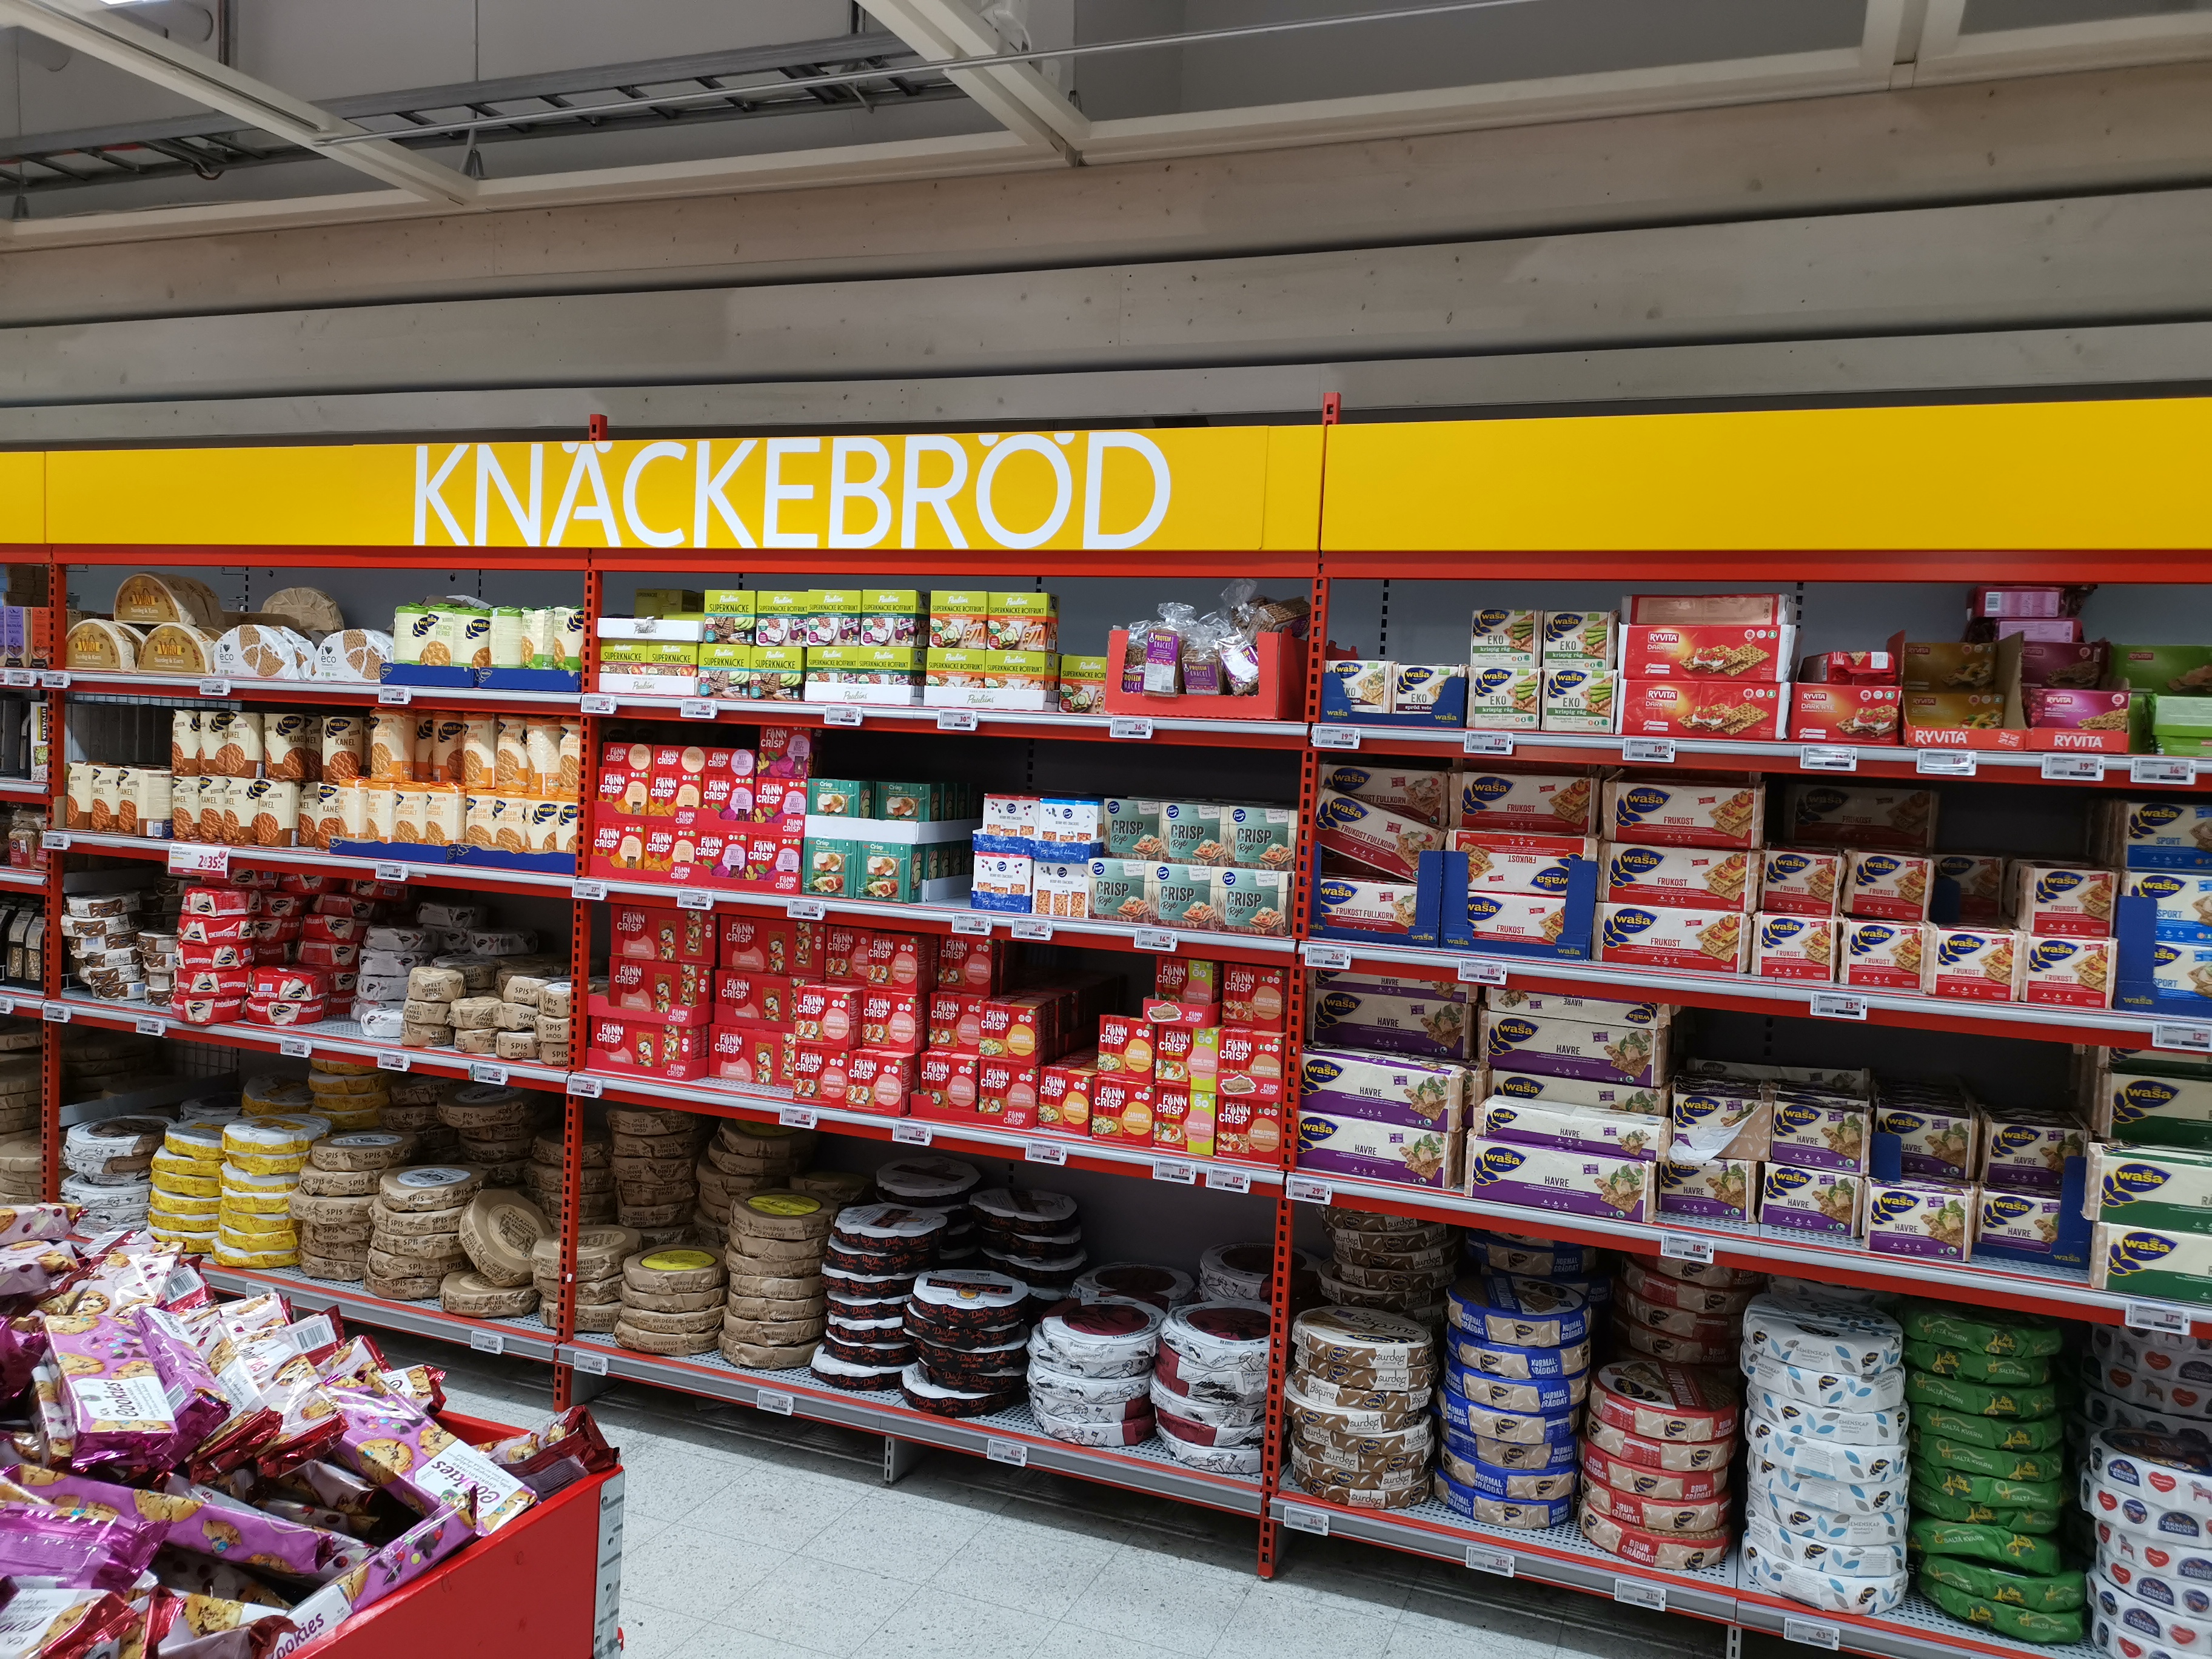
\includegraphics[width=0.4\linewidth]{images/knackebrot/original.jpg}
		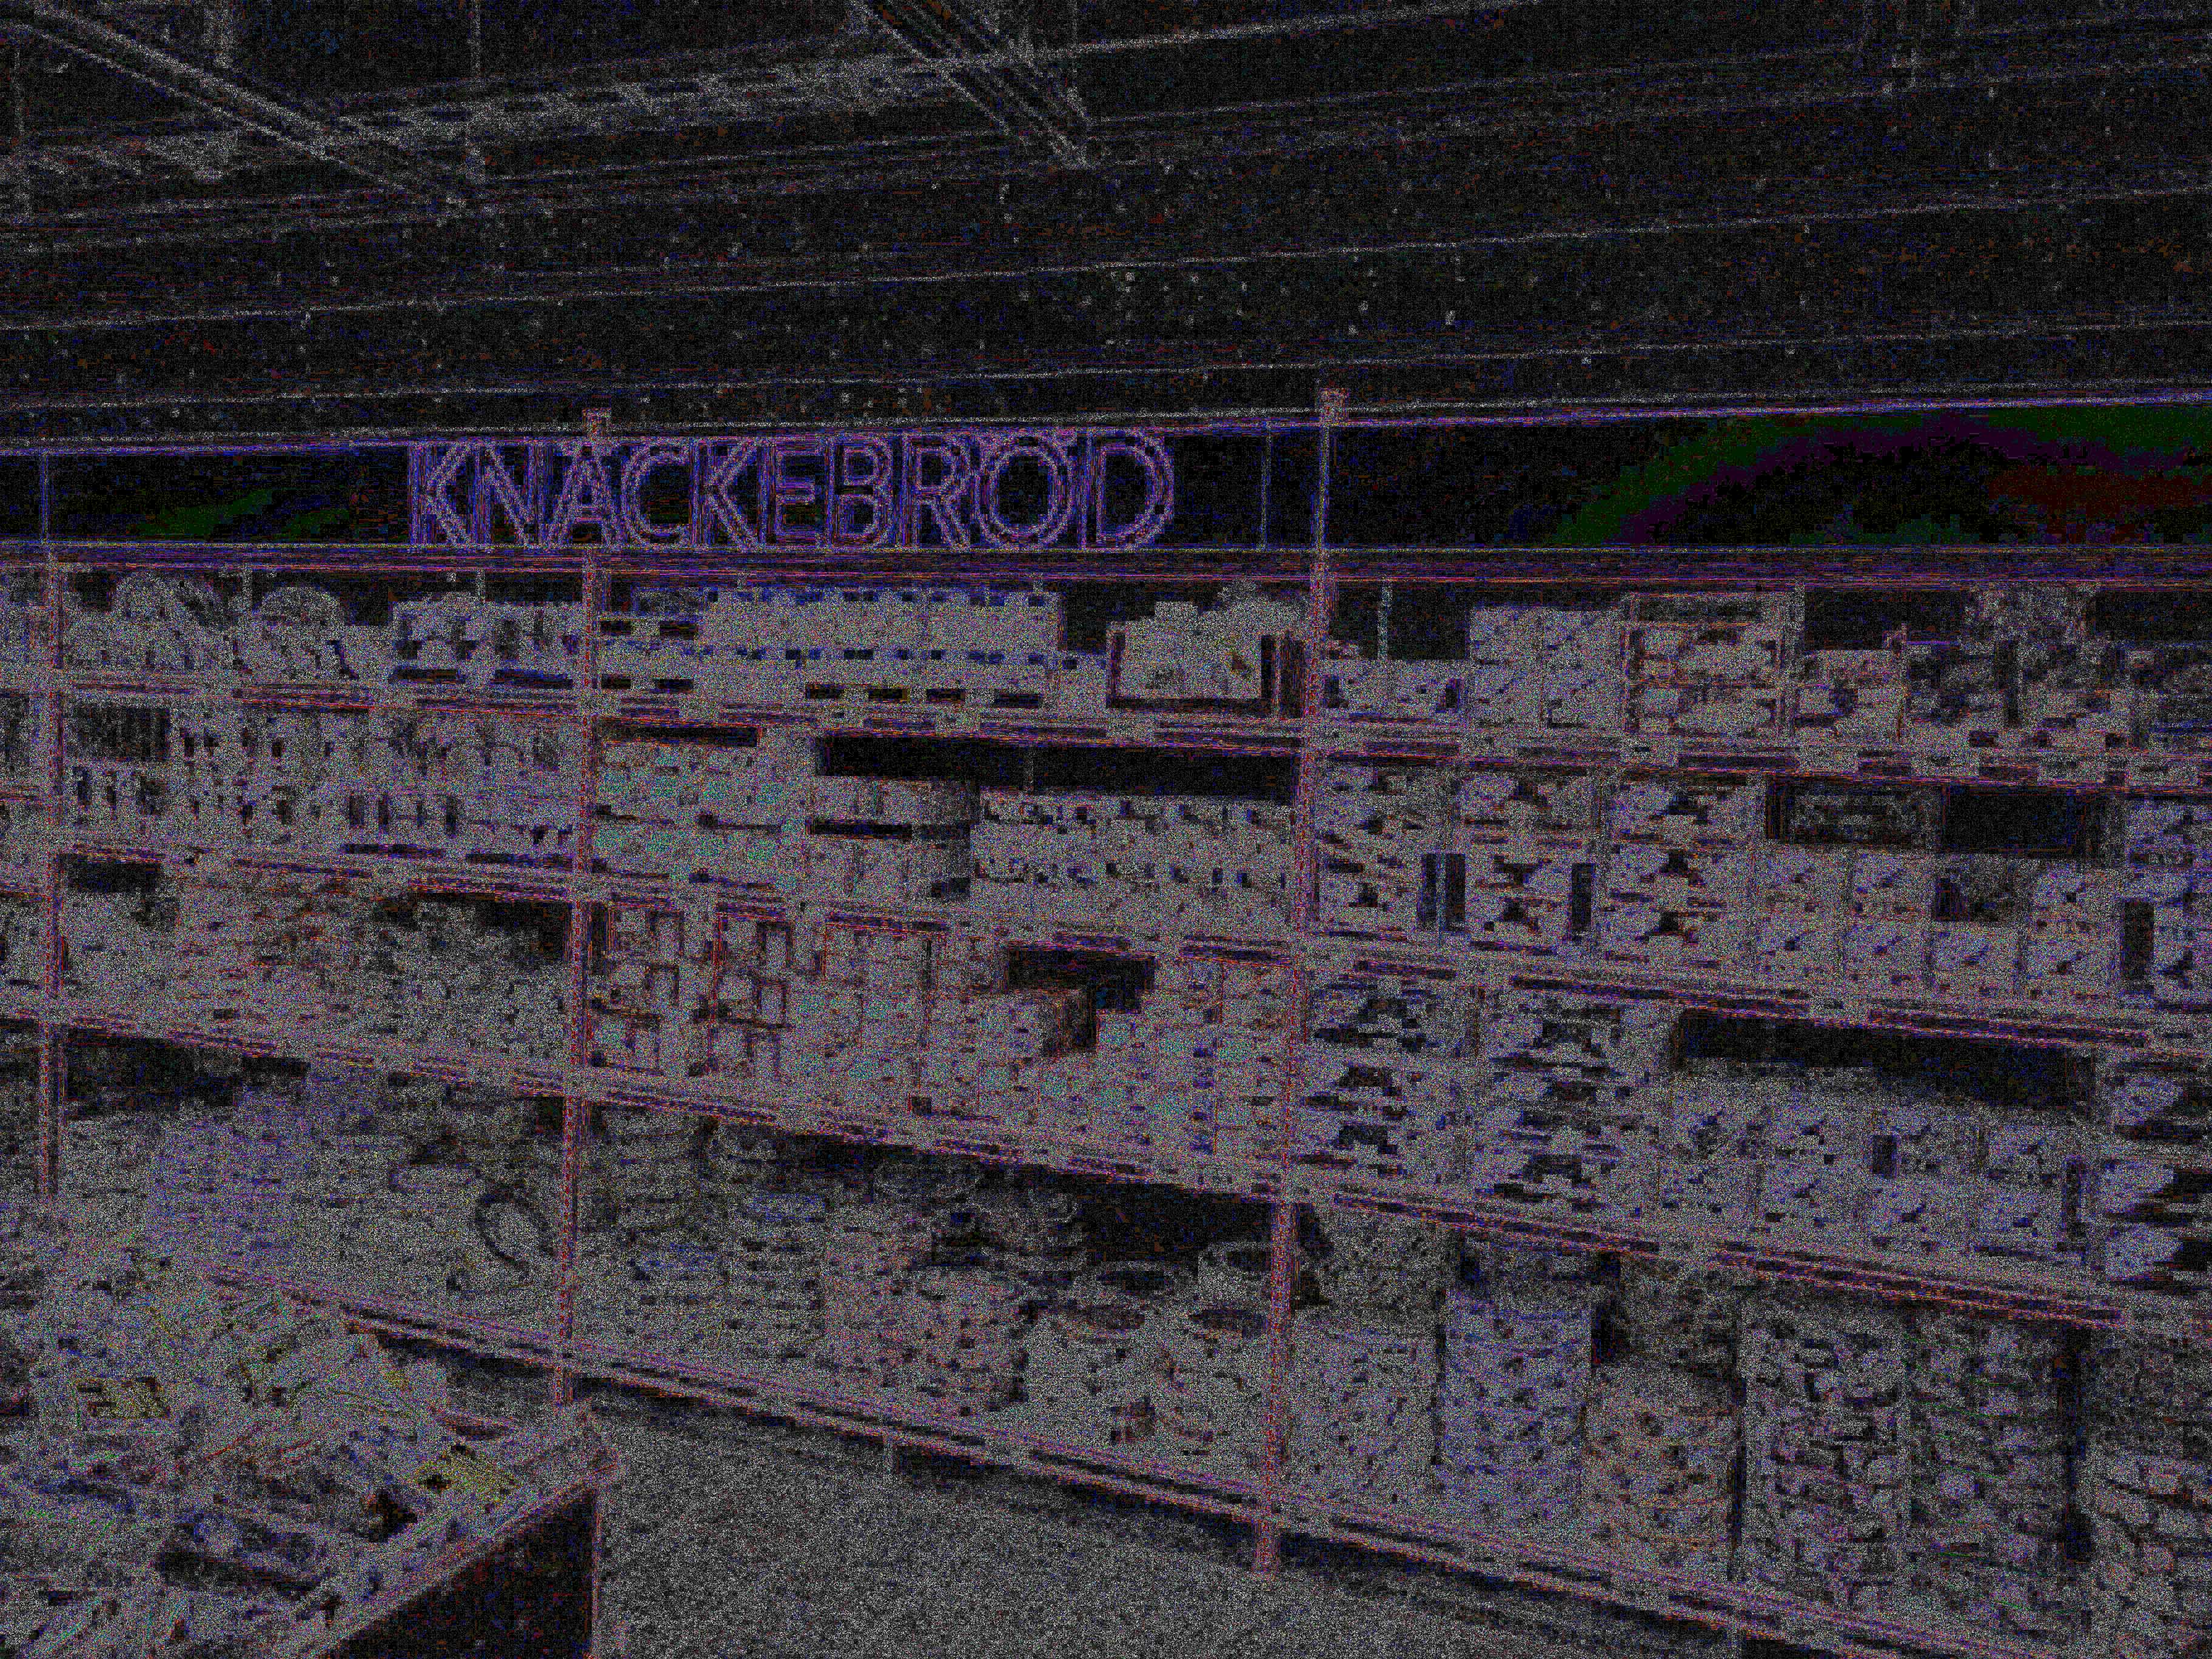
\includegraphics[width=0.4\linewidth]{images/knackebrot/originalELA.jpg}
		\caption{ELA mit Originalbild}
		\label{fig:elaOriginal}
	\end{center}
\end{figure}
\begin{figure}[H]
	\begin{center}
		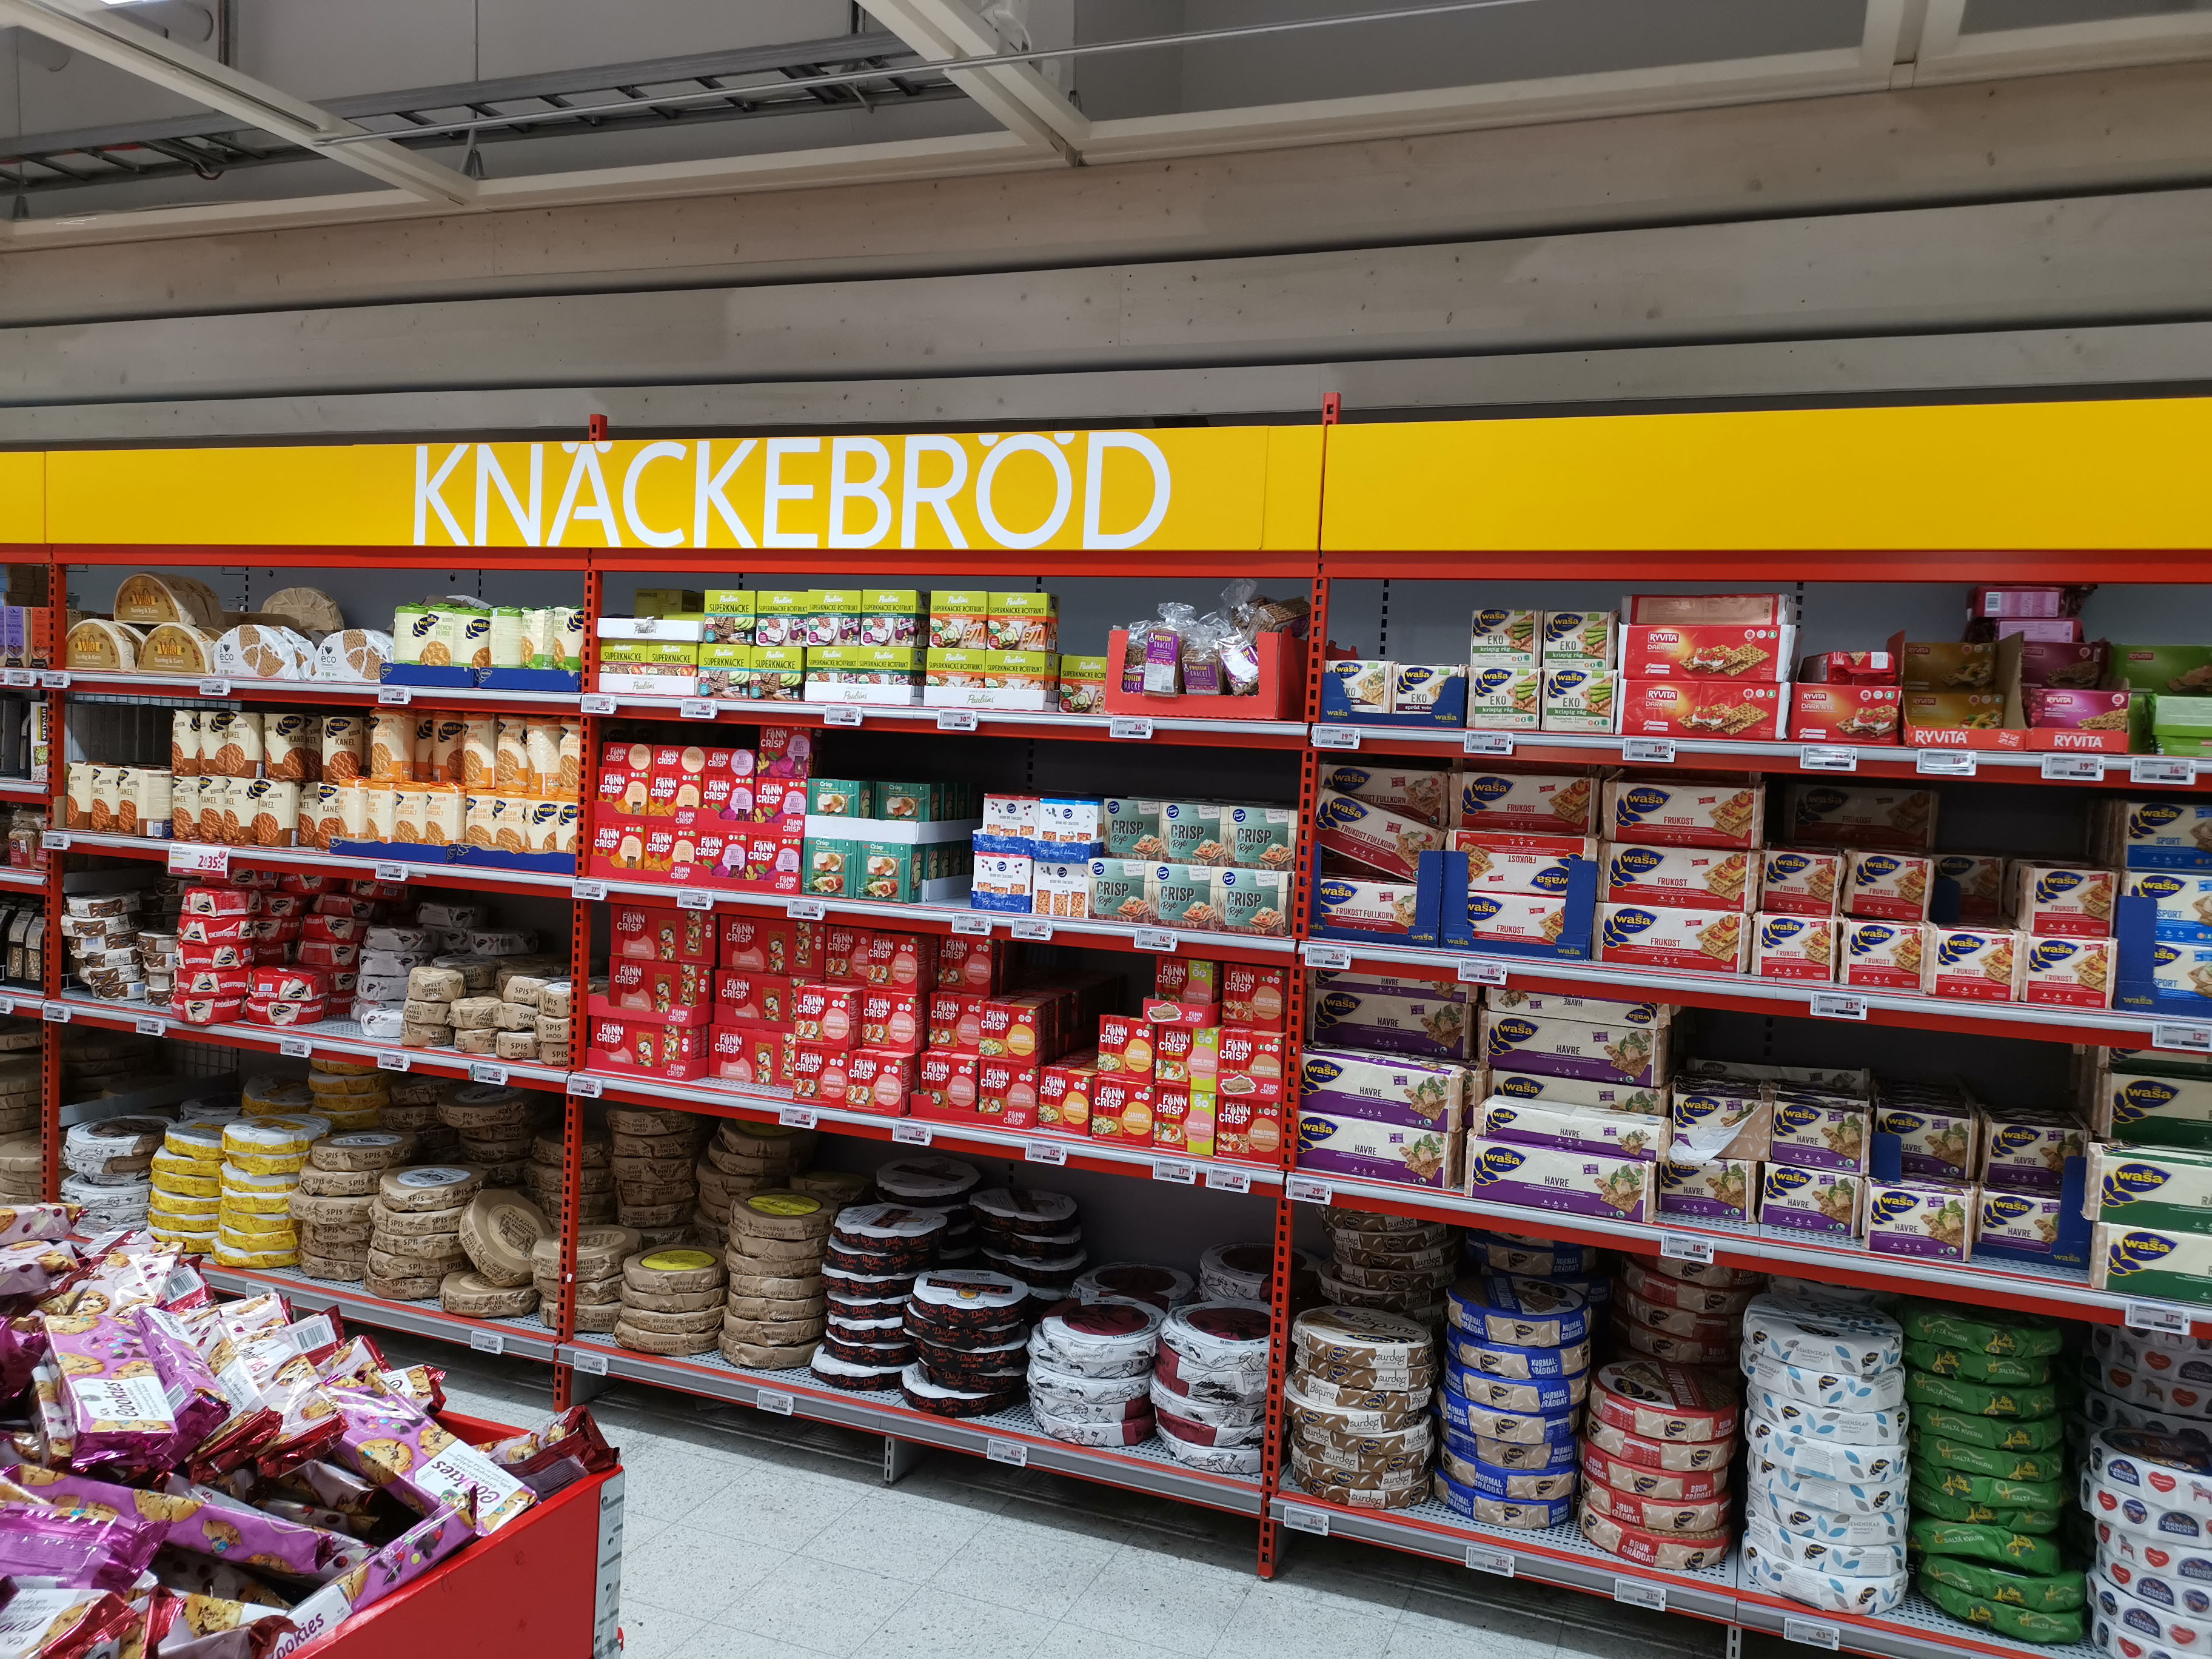
\includegraphics[width=0.4\linewidth]{images/knackebrot/photoshopQualityLevel8.jpg}
		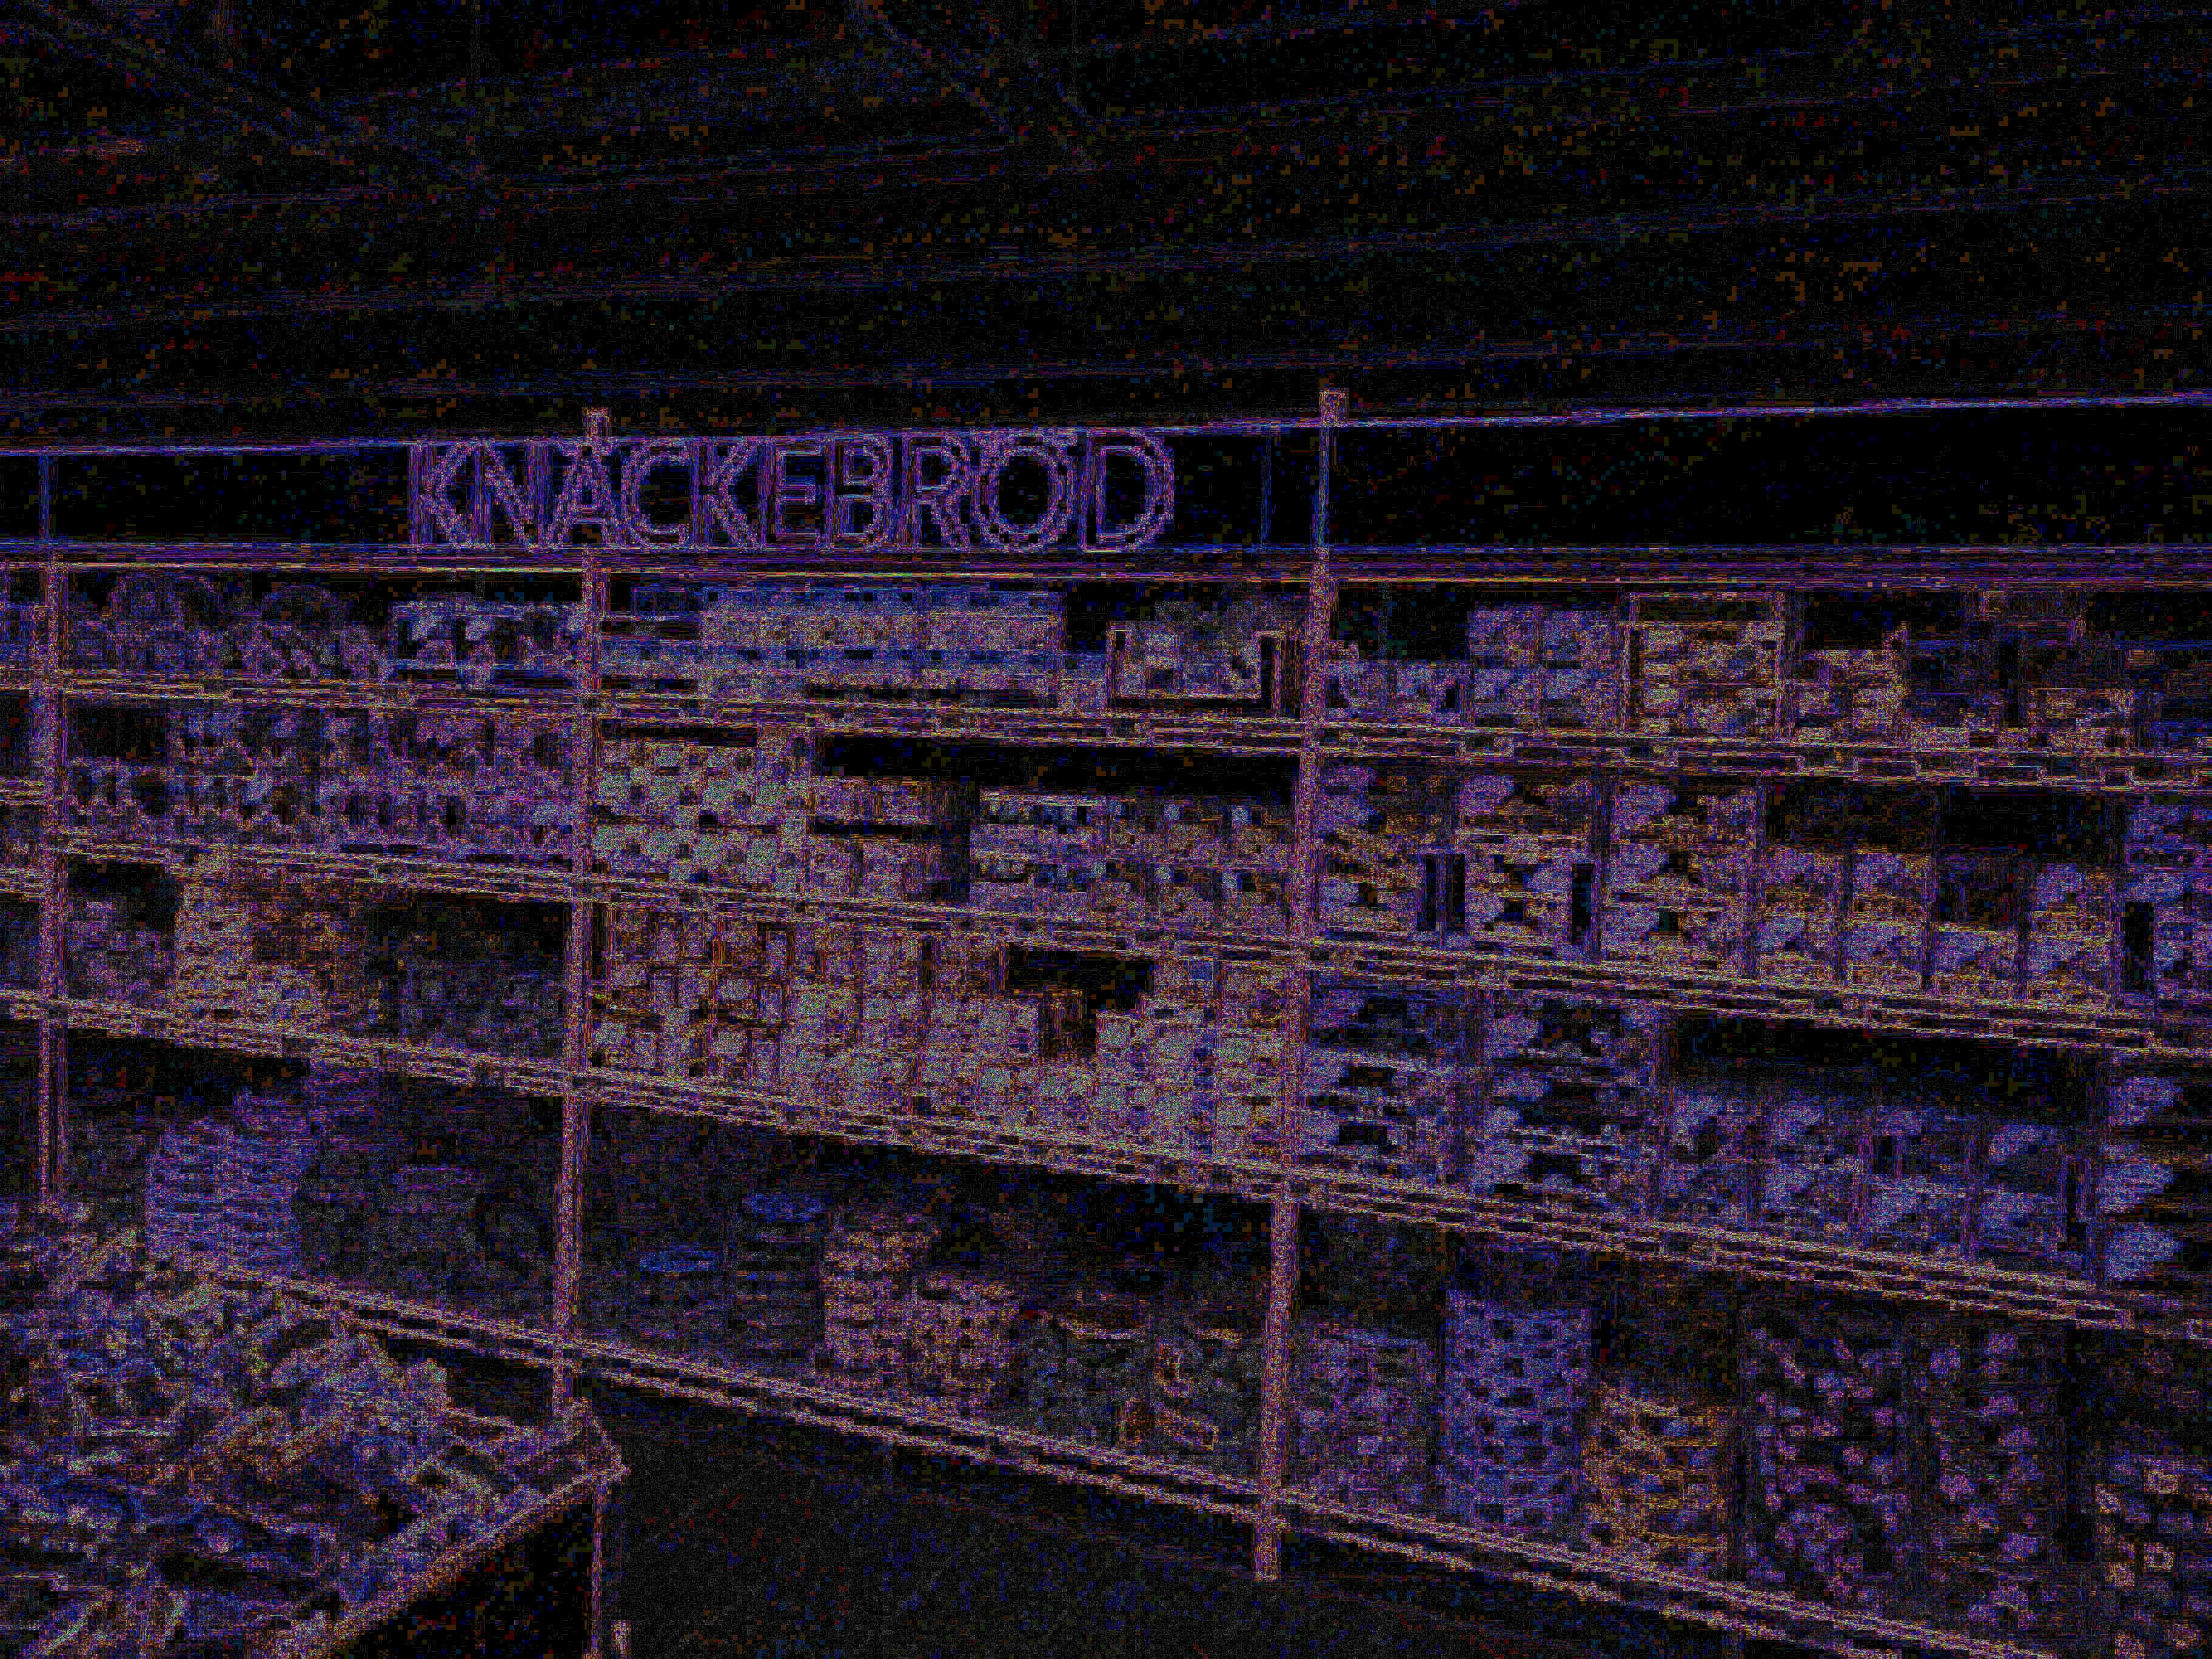
\includegraphics[width=0.4\linewidth]{images/knackebrot/photoshopQualityLevel8ELA.jpg}
		\caption{ELA nach speichern mit Adobe Photoshop 70\%}
		\label{fig:elaPhotoshop}
	\end{center}
\end{figure}
\begin{figure}[H]
	\begin{center}
		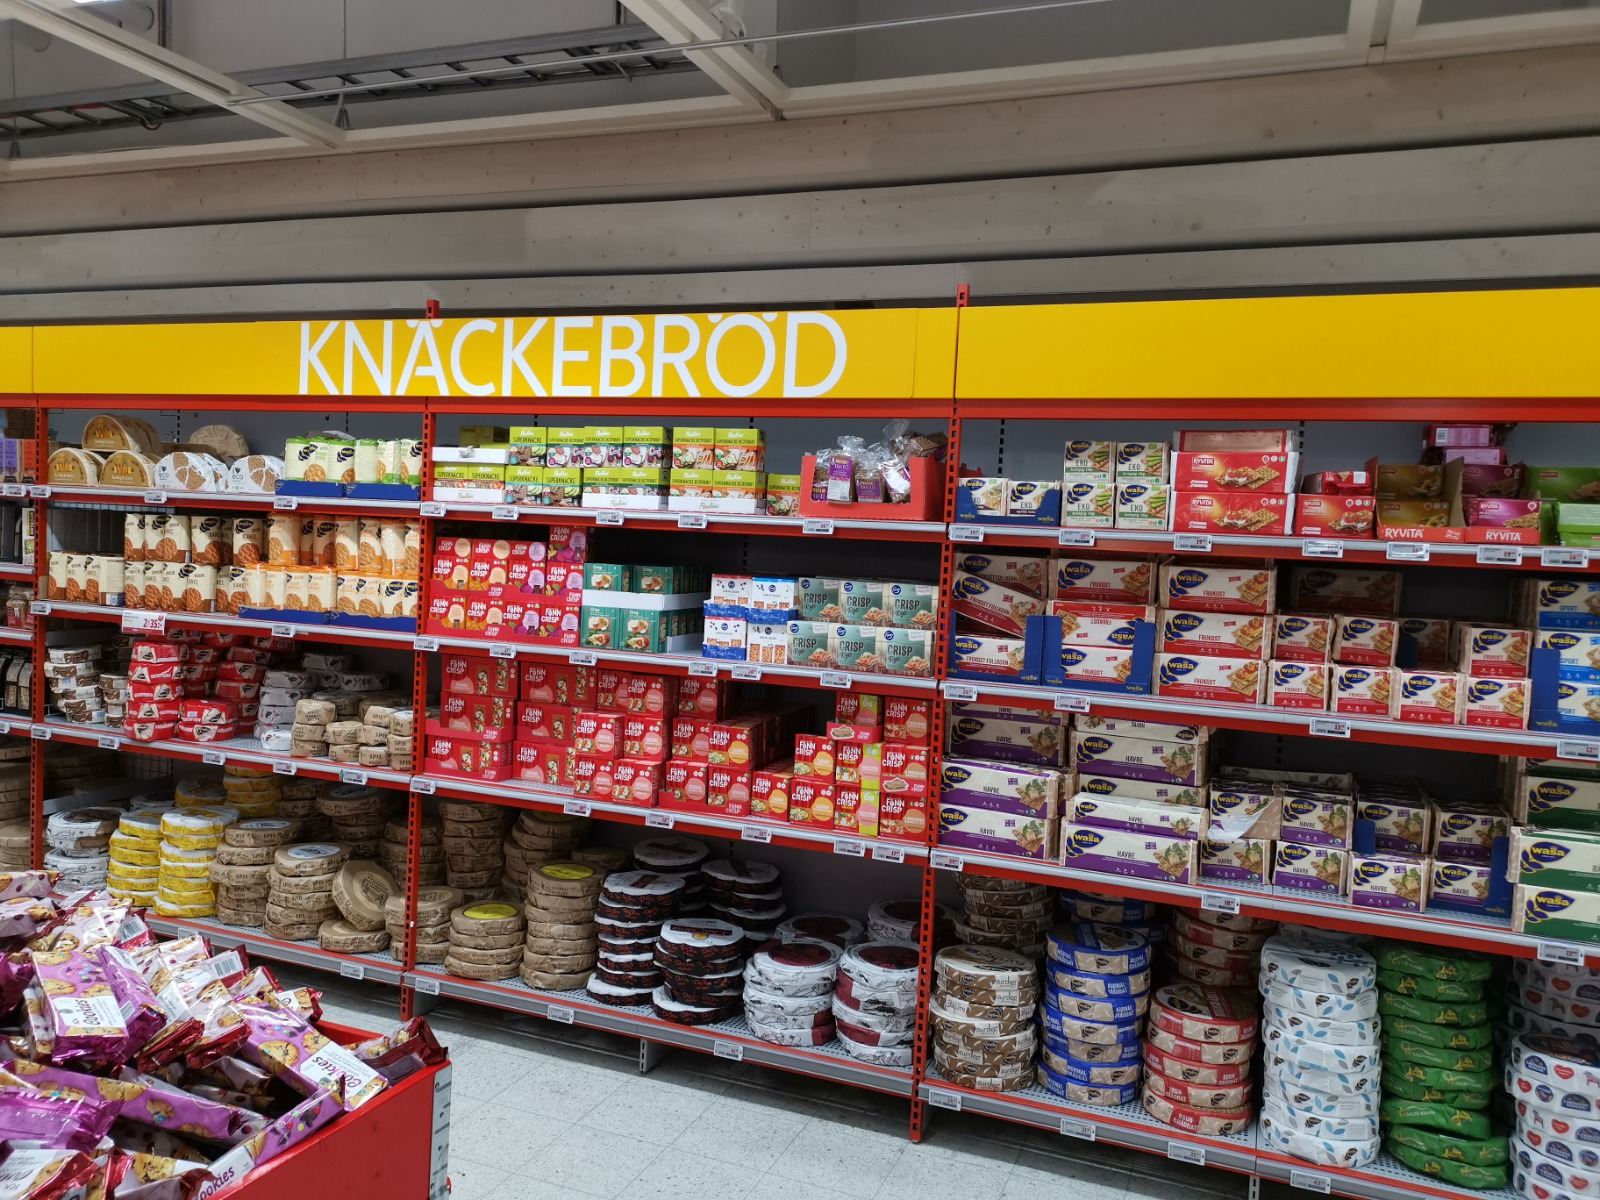
\includegraphics[width=0.4\linewidth]{images/knackebrot/whatsapp.jpg}
		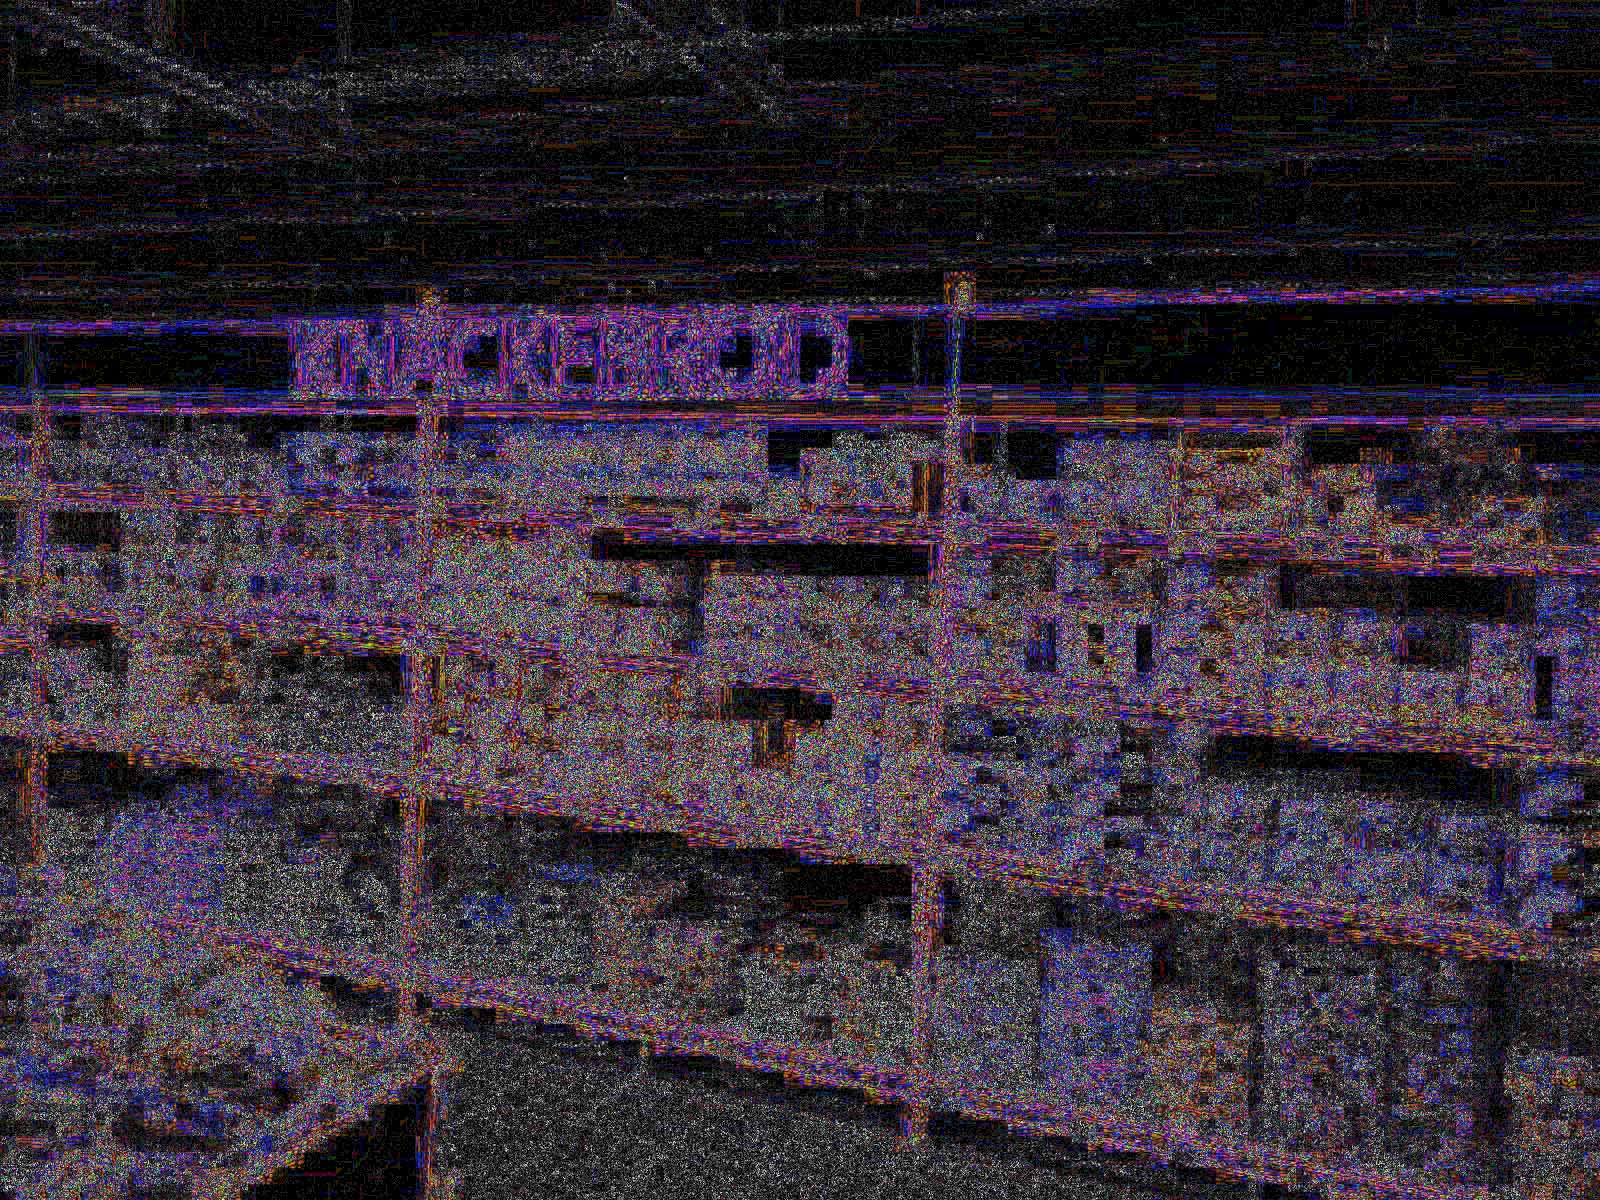
\includegraphics[width=0.4\linewidth]{images/knackebrot/whatsappELA.jpg}
		\caption{ELA nach versendet über Whatsapp}
		\label{fig:elaWhatsapp}
	\end{center}
\end{figure}

\autoref{fig:elaWhatsapp} zeigt das Bild welches in Adobe Photoshop komprimiert wurde und nachdem es über den Messenger Whatsapp versendet wurde. Bei diesem Schritt wurde zudem die Auflösung deutlich reduziert, was die Ursache dafür ist, dass es wieder heller im Vergleich zu dem Bild aus Adobe Photoshop ist. Durch die Änderung der Auflösung weisen die Bereiche welche vorher schon nahe an ihrem lokalen Fehlerminimum waren, also die dunklen, wieder eine große Menge an Veränderungen auf und erscheinen somit heller als im Schritt zuvor.

\section{Bildmanipulation}
Mit dem in \autoref{chap:mehrfachkompression} gewonnenen Erkenntnissen ist es nun möglich in einem generierten ELA-Bild Hinweise auf eine Bildmanipulation zu finden. Das Originalbild ist wieder in \autoref{fig:elaOriginal2} zu sehen und \autoref{fig:elafake} zeigt dieses mal eine Bildmontage bei welche an der linken Seite Knäckebrot durch Toilettenpapier ersetzt wurde, auf der rechten Seite Knäckebrot durch Seife ersetzt und über dem Regal noch ein Krümelmonster eingefügt wurde.\\
betrachtet man die Bildmanipulation für sich fällt dem Betrachter in den meisten Fällen vermutlich des Krümelmonster auf welches offensichtlich nicht echt ist. Bei genauerer Betrachtung fällt dann auch auf, dass Toilettenpapier und Seife auch nicht in das Bild passen.\\
Betrachtet man aber nur die Ausgabe der ELA, ist der erste Bildteil welcher ins Auge fällt der Teil mit dem Toilettenpapier, da dieser deutlich dunkler dargestellt wird als andere Teile des Regals. Das hat die Ursache, dass das eingefügte Bild vermutlich schon mehrfach komprimiert und abgespeichert wurde und es sich somit schon nahe am lokalen Kompressionsminimum befindet. Im mittlerer unveränderte Teil des Bildes befinden sich noch die Pixel vom Originalbild welche sich weit entfernt von ihrem lokalen Kompressionsminimum befinden. So kommt der hohe Kontrast zwischen diesen Bereich zustande welcher ein definitiver Hinweis darauf ist, dass es sich hier um eine Bildmontage handelt.

\begin{figure}[H]
	\begin{center}
		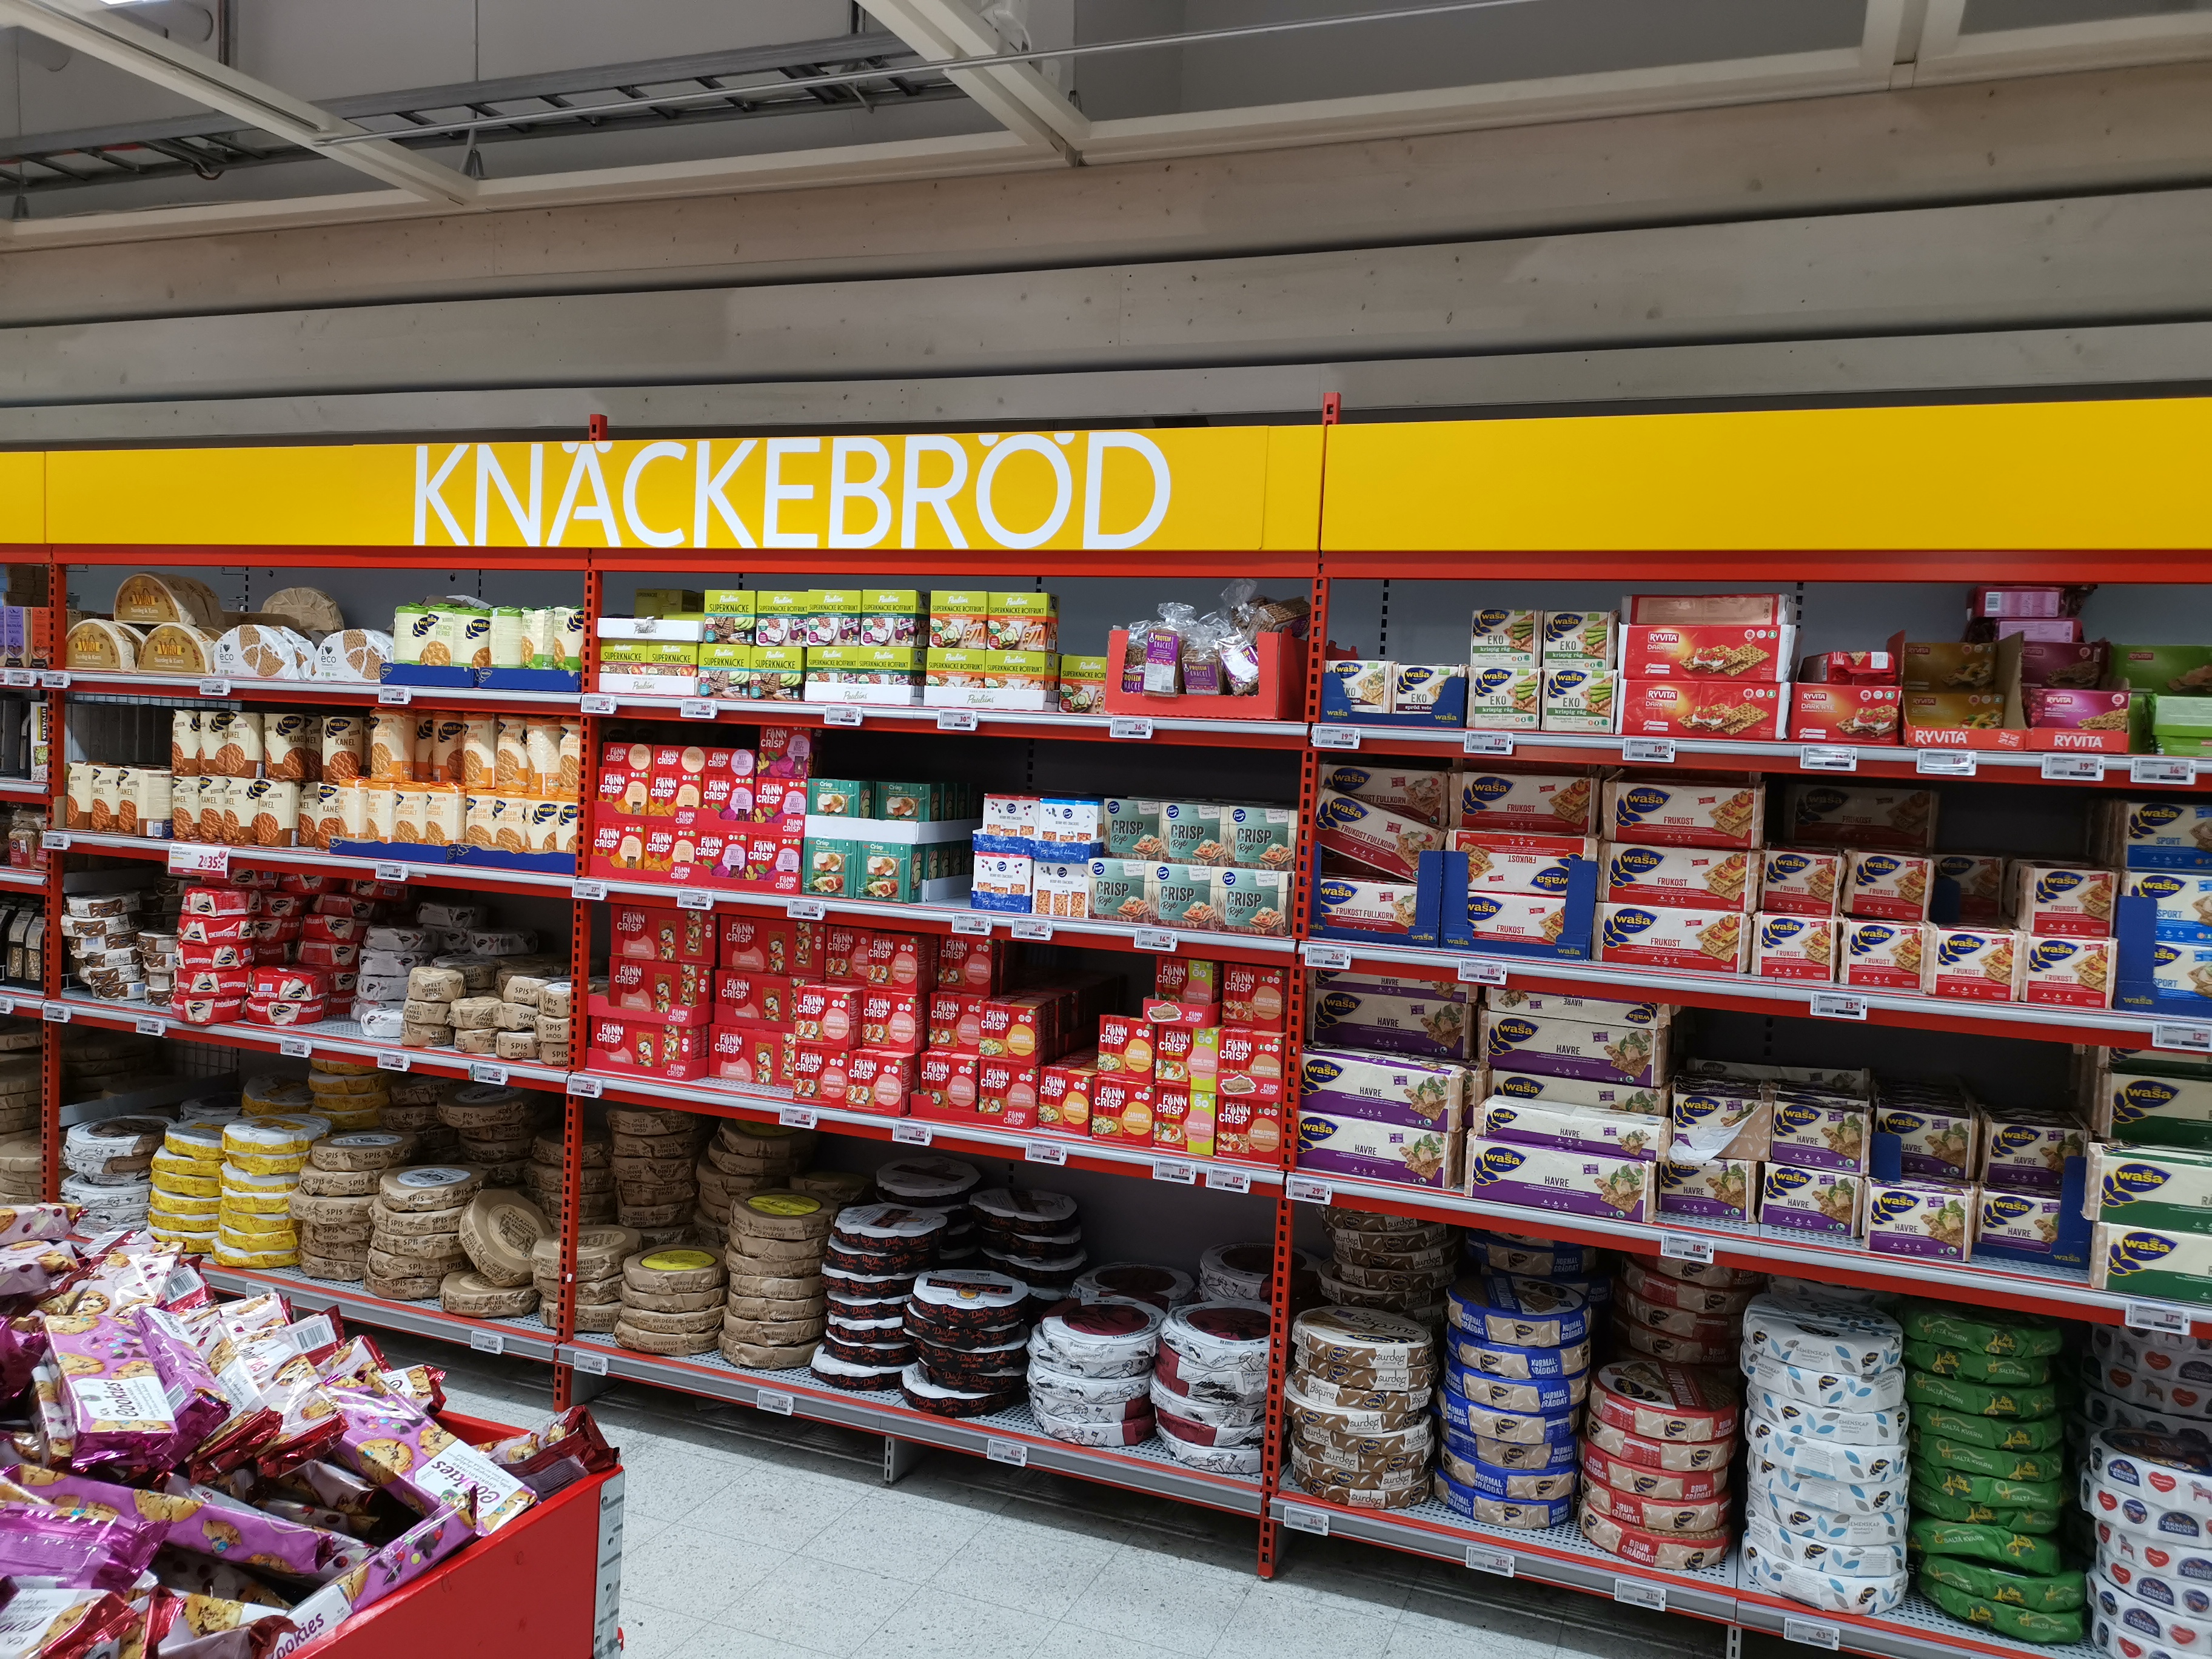
\includegraphics[width=0.4\linewidth]{images/knackebrot/original.jpg}
		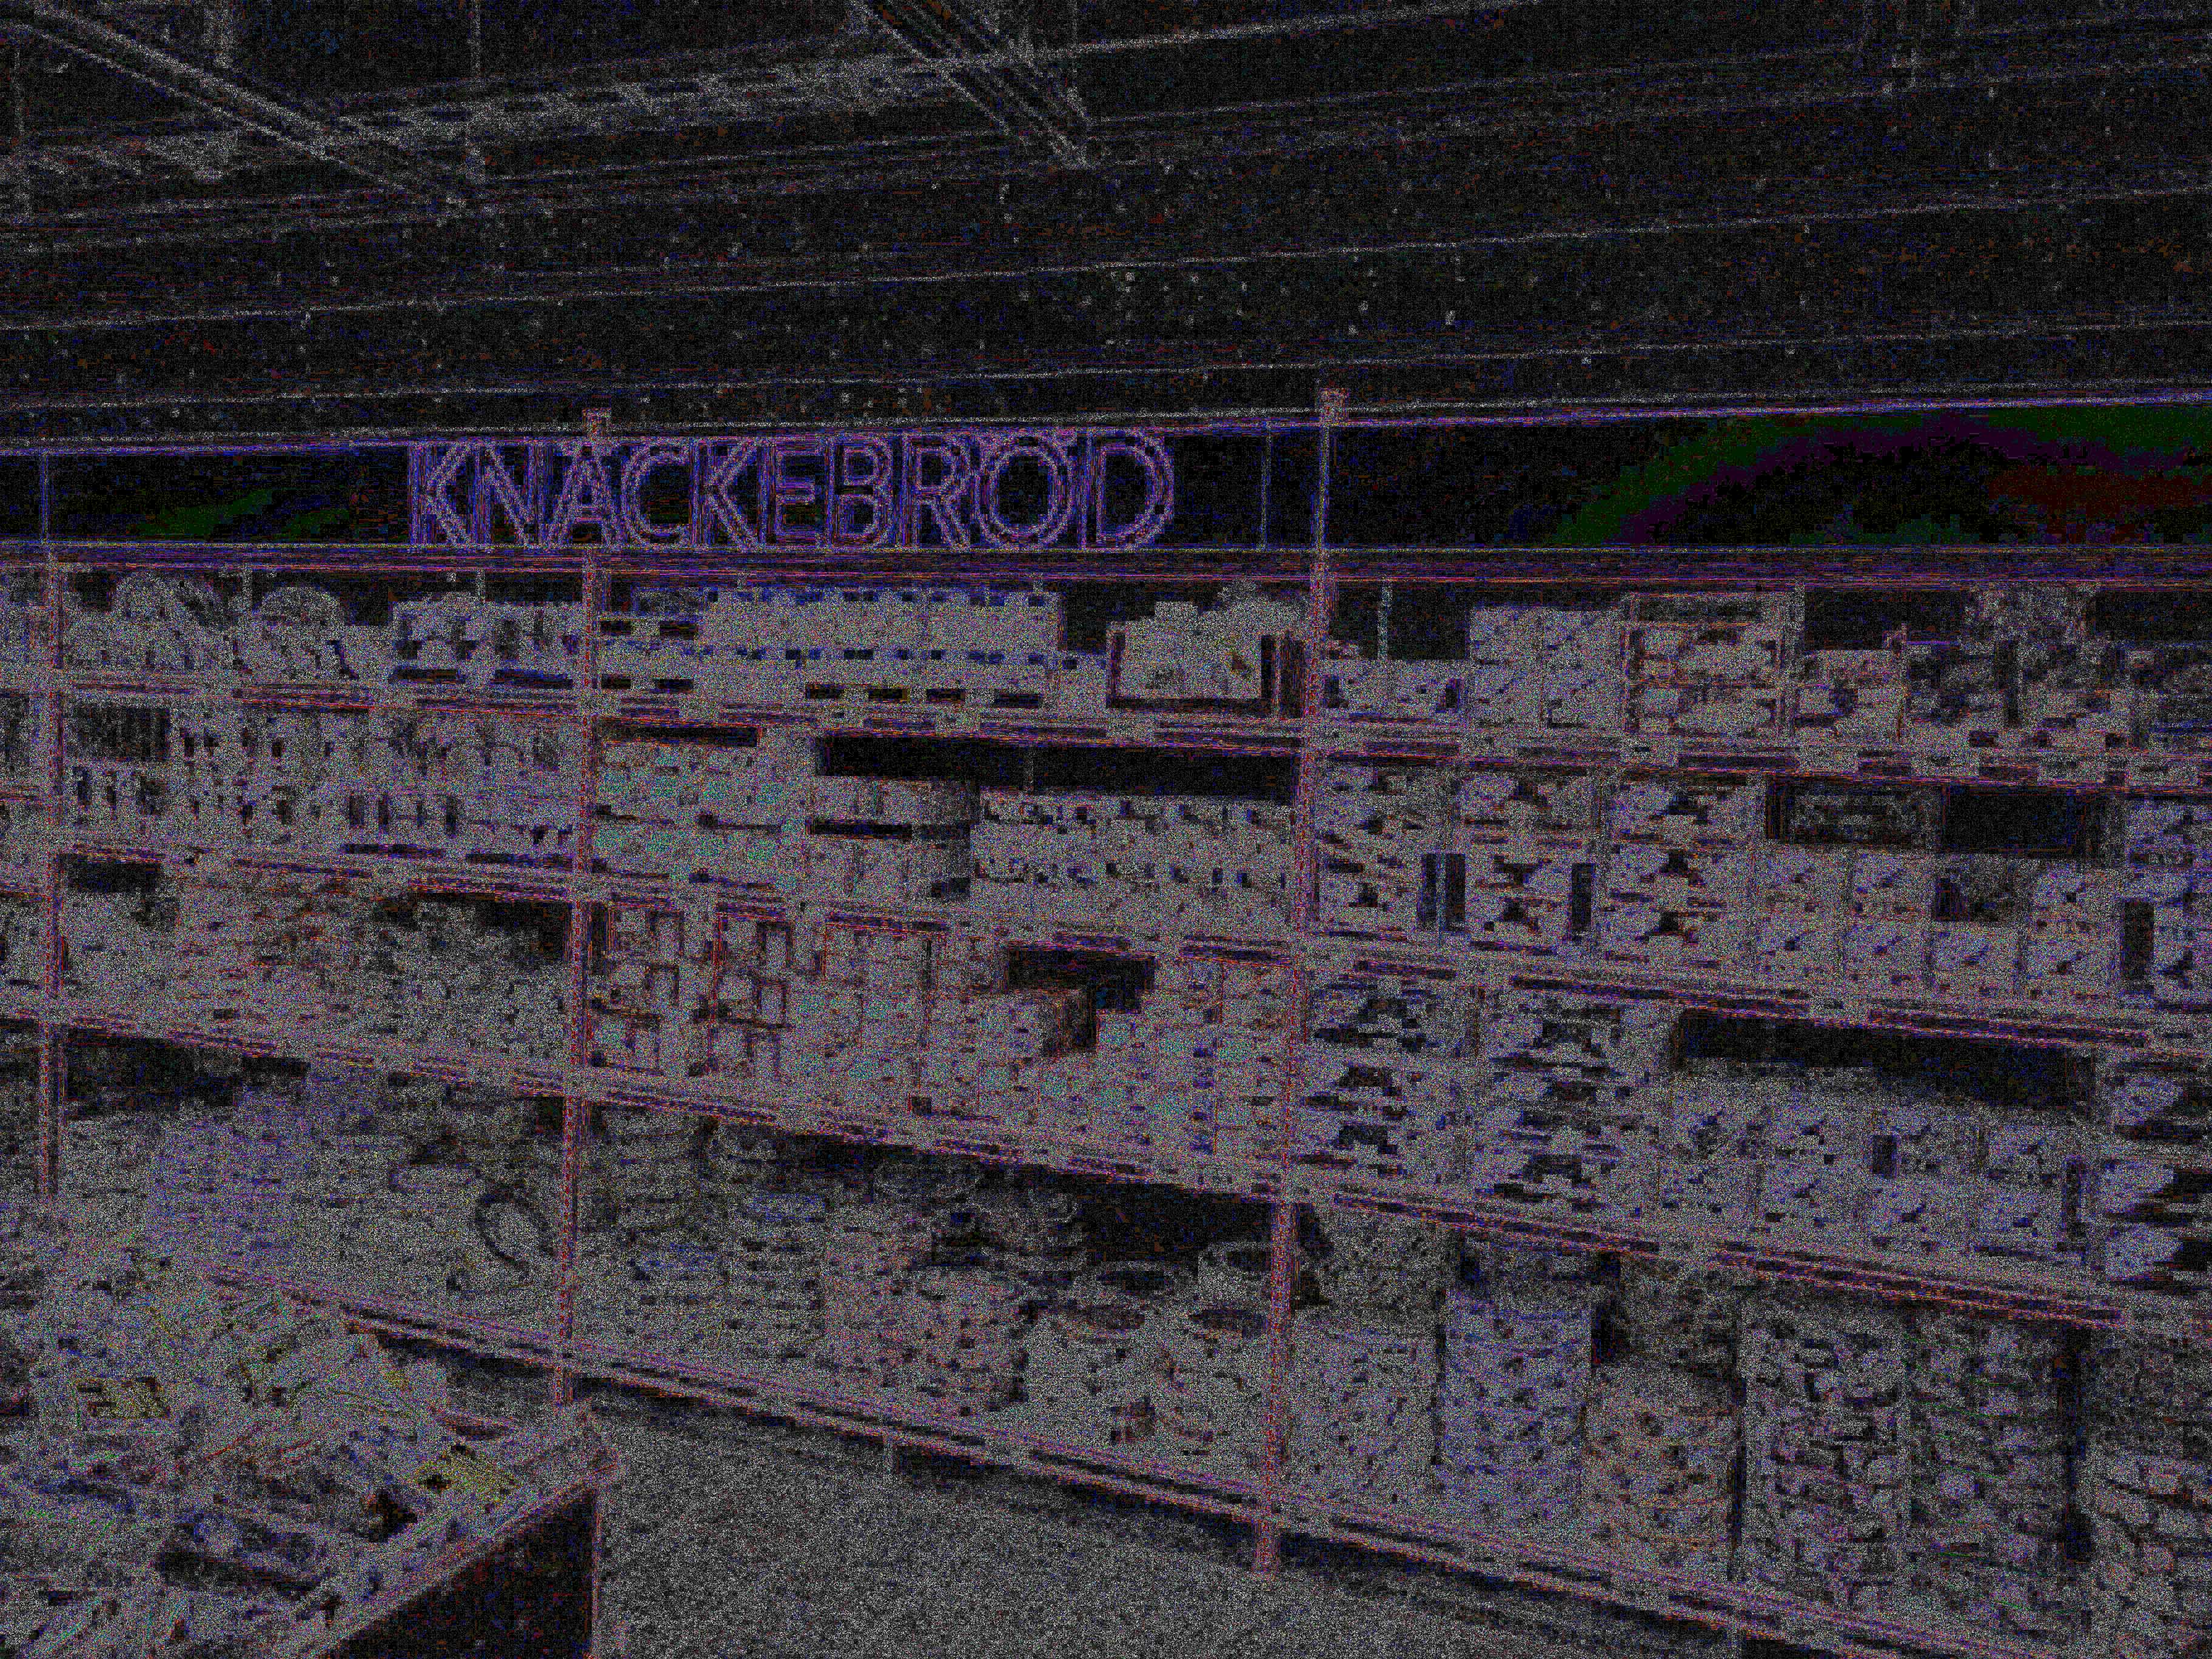
\includegraphics[width=0.4\linewidth]{images/knackebrot/originalELA.jpg}
		\caption{ELA mit Originalbild}
		\label{fig:elaOriginal2}
	\end{center}
\end{figure}
\begin{figure}[H]
	\begin{center}
		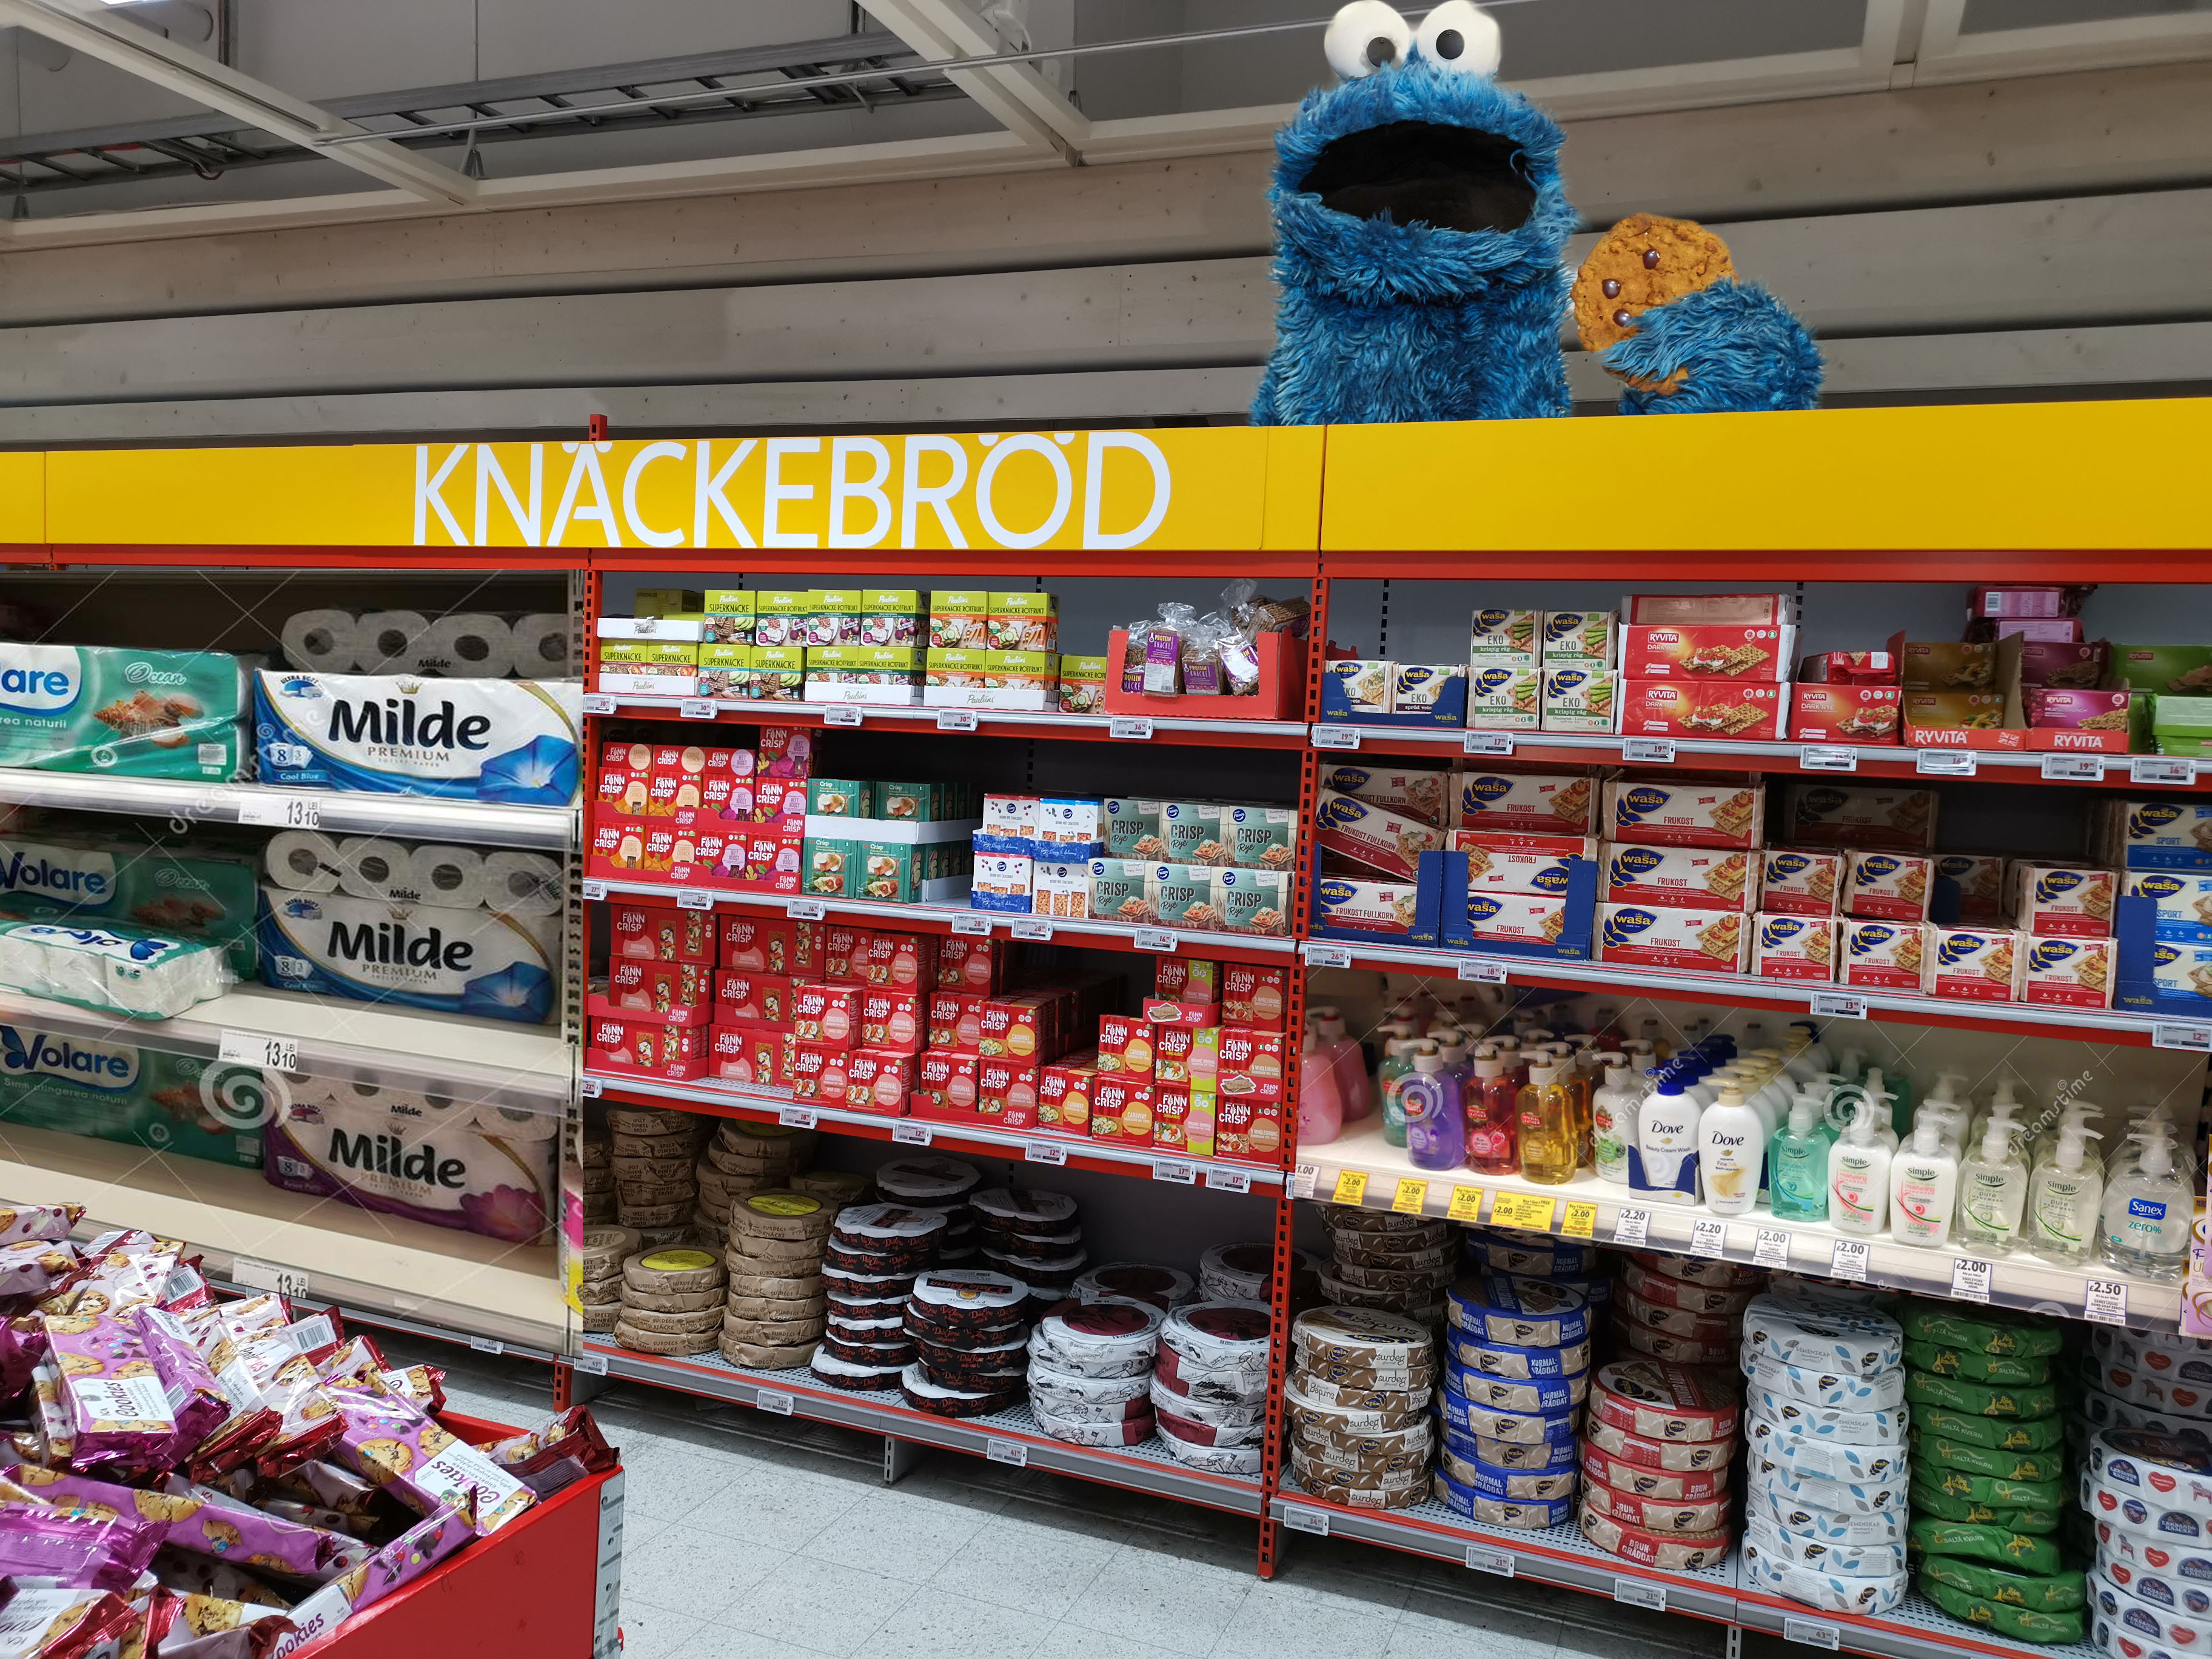
\includegraphics[width=0.4\linewidth]{images/knackebrot/fake.jpg}
		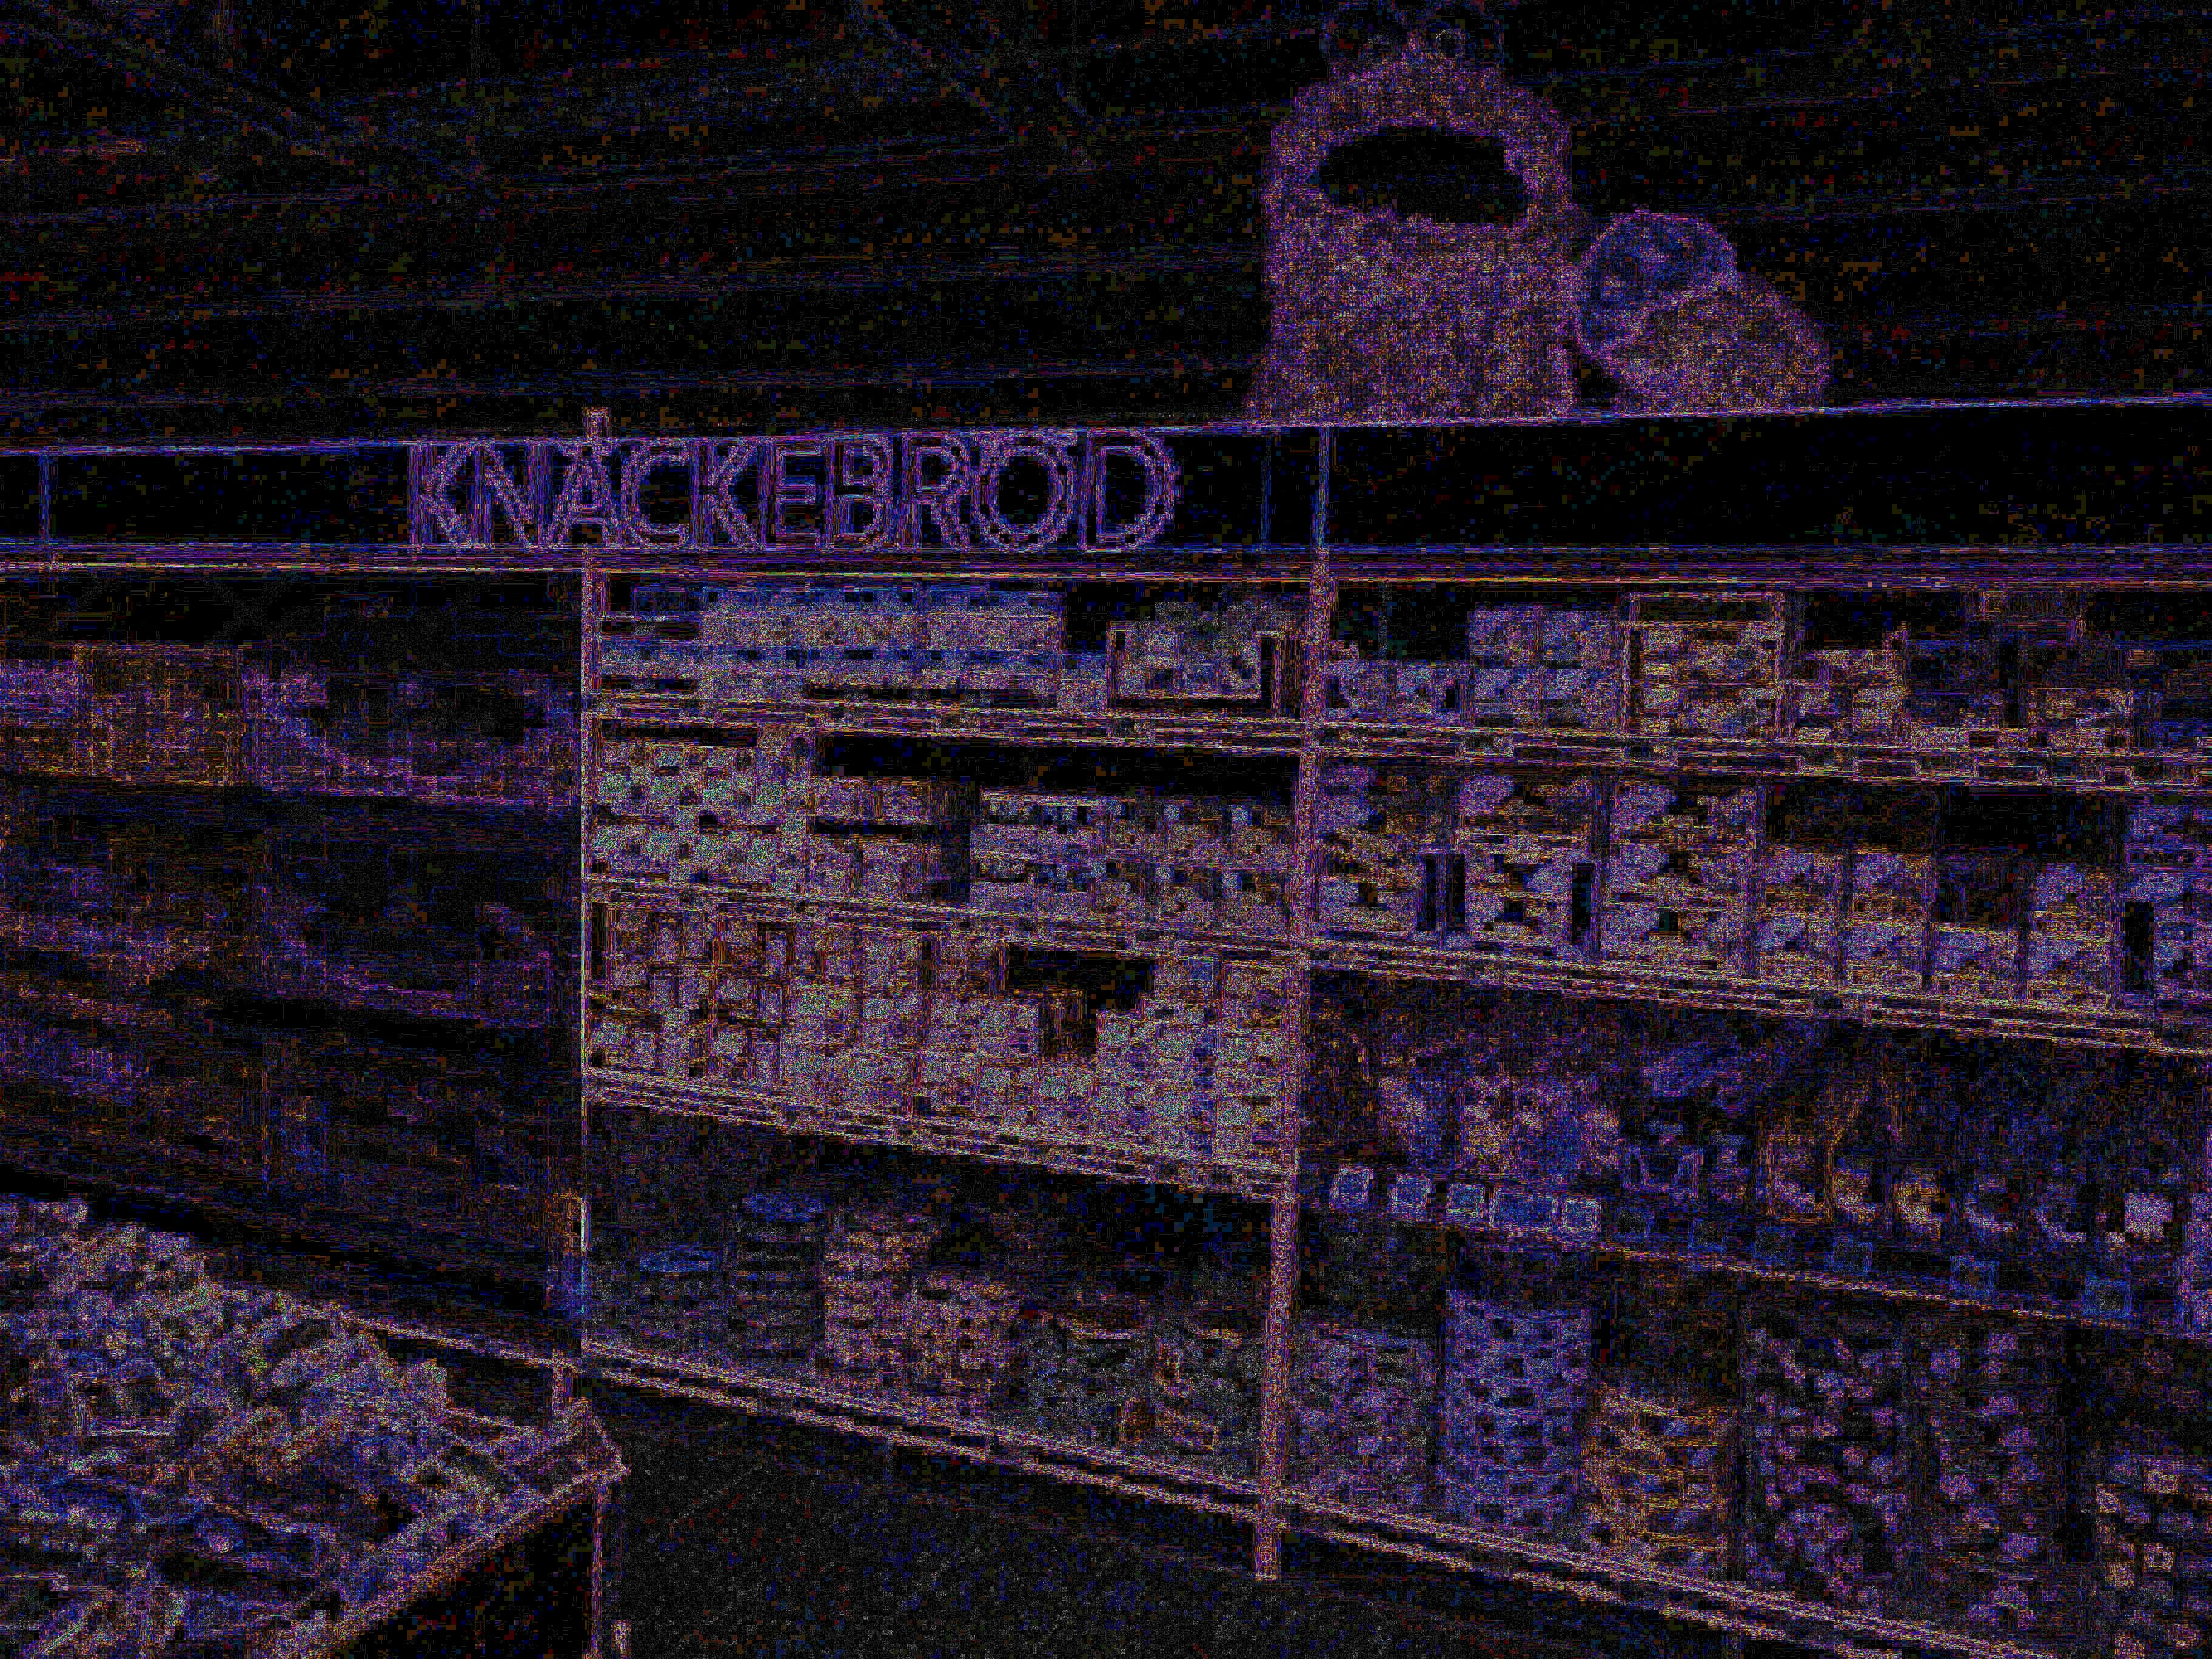
\includegraphics[width=0.4\linewidth]{images/knackebrot/fakeELA.jpg}
		\caption{Bildmontage}
		\label{fig:elafake}
	\end{center}
\end{figure}

\chapter{Zusammenfassung}
dtzjtukjztukzukzukuk











	
	\pagenumbering{Roman}
	\setcounter{page}{\thesavepage}
	

%\addcontentsline{toc}{chapter}{Anhang}
%\addcontentsline{toc}{chapter}{Index}
%\printindex


\addcontentsline{toc}{chapter}{Literaturverzeichnis}
\bibliographystyle{IEEEtran}
\bibliography{bericht}


\renewcommand{\appendixpagename}{Anhang}
\renewcommand{\appendixtocname}{Anhang}

% Ab hier beginnt der Anhang
\appendix
\begin{appendices}
	\chapter{Anhang}

	\todo[inline]{Gibt es einen Appendix?}	
\end{appendices}
	
	\listoftodos
	\todo[inline]{List of Todos entfernen}
\end{document}
